% !TEX program = xelatex
\documentclass[UTF8,fontset=fandol,a4paper,11pt]{ctexart}
\usepackage[margin=21mm,top=23mm,bottom=22mm,headheight=16pt]{geometry}
\usepackage{amsmath,amssymb,mathtools,bm}
\usepackage{tikz}
\usetikzlibrary{arrows.meta,calc,angles,quotes,patterns,decorations.pathmorphing}
\usepackage{xcolor,booktabs,array,longtable,enumitem,fancyhdr,needspace}
\usepackage[unicode,hidelinks]{hyperref}
\definecolor{ink}{HTML}{24343C}
\definecolor{accent}{HTML}{166A70}
\definecolor{muted}{HTML}{65747A}
\definecolor{rulegray}{HTML}{D4DDE0}
\definecolor{warm}{HTML}{966037}
\color{ink}
\setlength{\parindent}{2em}
\setlength{\parskip}{4pt}
\linespread{1.12}
\AtBeginDocument{\setlength{\abovedisplayskip}{6pt plus 2pt minus 1pt}
\setlength{\belowdisplayskip}{6pt plus 2pt minus 1pt}
\setlength{\abovedisplayshortskip}{0pt plus 1pt}
\setlength{\belowdisplayshortskip}{4pt plus 1pt}}
\setlist[enumerate]{label=(\arabic*),leftmargin=2.3em,itemsep=3pt,topsep=4pt}
\setlist[itemize]{leftmargin=2em,itemsep=2pt,topsep=4pt}
\allowdisplaybreaks[1]
\setlength{\emergencystretch}{2em}
\setcounter{secnumdepth}{0}
\providecommand{\tightlist}{\setlength{\itemsep}{0pt}\setlength{\parskip}{0pt}}
\ctexset{section={format=\Large\bfseries\color{accent},beforeskip=10pt,afterskip=9pt},
subsection={format=\normalsize\bfseries\color{accent},beforeskip=10pt,afterskip=4pt},
subsubsection={format=\normalsize\bfseries,beforeskip=8pt,afterskip=3pt}}
\pagestyle{fancy}
\fancyhf{}
\fancyhead[L]{\small\color{muted}物理学难题集萃}
% 页眉仅保留书名；版本名称只在封面显示。
\fancyfoot[L]{\small\color{muted}\chapterlabel}
\fancyfoot[R]{\small\thepage}
\renewcommand{\headrulewidth}{0.4pt}
\renewcommand{\footrulewidth}{0pt}
\newcommand{\dd}{\mathop{}\!\mathrm{d}}
\newcommand{\vect}[1]{\bm{#1}}
\newcommand{\tagline}[1]{\noindent{\small\color{muted}#1}\par}
\newcommand{\result}[1]{\begin{equation*}\boxed{#1}\end{equation*}}
\newcommand{\figcaption}[1]{\par\vspace{2pt}{\small\color{muted}#1}\par}
\newcommand{\teach}[2]{\Needspace{4\baselineskip}\subsection*{讲解要点与追问}#1\par\smallskip\noindent\textbf{追问：}#2\par}
\newcommand{\workarea}{\par\vspace{7mm}\noindent{\small\color{muted}作答区}\par\vspace{4mm}
\noindent\textcolor{rulegray}{\rule{\linewidth}{0.3pt}}\par\vspace{16mm}
\noindent\textcolor{rulegray}{\rule{\linewidth}{0.3pt}}\par\vspace{16mm}
\noindent\textcolor{rulegray}{\rule{\linewidth}{0.3pt}}\par\vspace{16mm}
\noindent\textcolor{rulegray}{\rule{\linewidth}{0.3pt}}}
\tikzset{axis/.style={-{Stealth[length=2mm]},thin,color=muted},
motion/.style={-{Stealth[length=2.3mm]},thick,color=accent},
force/.style={-{Stealth[length=2.3mm]},thick,color=warm},
traj/.style={thick,color=accent},guide/.style={dashed,thin,color=muted},
object/.style={thick,color=ink},every node/.style={font=\small}}\widowpenalty=10000\clubpenalty=10000\displaywidowpenalty=10000

\newcommand{\chapterlabel}{第五章\quad 静力平衡}
\hypersetup{pdftitle={第五章 静力平衡·学生解答版},pdfauthor={},pdfsubject={第五章第1--12题}}
\begin{document}
\pdfbookmark[0]{第五章 静力平衡}{cover}
\thispagestyle{empty}
\vspace*{20mm}
\noindent{\Huge\bfseries 物理学难题集萃}\par\vspace{8mm}
\noindent{\LARGE 第五章\quad 静力平衡}\par\vspace{10mm}
\noindent{\Large\color{accent}学生解答版}\par\vspace{8mm}
\noindent\textcolor{accent}{\rule{\linewidth}{1pt}}\par\vspace{8mm}
\noindent 第 1--12 题\par\vspace{5mm}
\noindent 完整推导、图示分析与条件讨论。\par
\vfill\clearpage
\pdfbookmark[1]{题目目录}{contents}
\section*{题目目录}
\begin{longtable}{@{}>{\color{accent}\bfseries}r p{120mm}@{}}
\toprule 题号 & 题目\\\midrule
1 & 圆锥面上链环的张力 \\
2 & 水平杆靠墙的摩擦条件 \\
3 & 竖杆受水平力的防滑条件 \\
4 & 半球凹面内的均匀细杆 \\
5 & 三圆柱堆放的摩擦下限 \\
6 & 斜木板上三球的支承 \\
7 & 分段悬线的平衡与提升功 \\
8 & 浮子与插杆的稳定性 \\
9 & 五杆悬挂的平衡形状 \\
10 & 厚木板在圆柱上的稳定性 \\
11 & 菱形木条与圆盘的平衡 \\
12 & 细绳张力与悬链线 \\
\bottomrule\end{longtable}


\clearpage

\pdfbookmark[2]{第 1 题 圆锥面上链环的张力}{q1}

\section*{第 1 题\quad 圆锥面上链环的张力}

\tagline{M-05-01}

顶角为 $\alpha$ 的圆锥体竖直固定，顶点在上。质量为 $m$、质量分布均匀的链环水平套在圆锥面上，处于静止状态。忽略链环与圆锥面之间的摩擦，$0<\alpha<\pi$。求链环中的张力。

\begin{center}\begin{minipage}{\linewidth}\centering
\begin{tikzpicture}
\draw[object] (-2,0)--(0,4)--(2,0);\draw[guide] (0,0)--(0,4);\draw[object] (0,1.6) ellipse (1.2 and .32);\draw (0,3.3) arc(-90:-116.57:.7);\node at (-.45,3.15) {$\alpha/2$};\node[right] at (1.3,1.6) {$m$};\node[below] at (0,-.1) {链环水平};
\end{tikzpicture}
\figcaption{图 5.1\quad 水平链环套在圆锥外侧，锥面母线与竖直轴夹角为 $\alpha/2$。}
\end{minipage}\end{center}

\Needspace{5\baselineskip}\subsection*{解答}

\textbf{链元的质量与支持力。}整环的水平支持力相互抵消。截取链弧后，切口处的张力成为该段外力，才能由受力求得。取对应圆心角 $\dd\varphi$ 的短链元。设链环半径为 $r$，质量均匀，故
\[
 \dd s=r\dd\varphi,\qquad
 \dd m=\frac{m}{2\pi r}\dd s=\frac{m}{2\pi}\dd\varphi.
\]
记圆锥半顶角为 $\beta=\alpha/2$。解图5.1A中，支持力 $N$ 垂直于锥面，方向朝外且向上。其竖直分量承受链元重力：
\[
 N\sin\beta=\dd m\,g,
 \qquad N=\frac{mg}{2\pi\sin\beta}\dd\varphi.
\]
\begin{center}\begin{minipage}{\linewidth}\centering
\begin{tikzpicture}
\draw[object](-1.5,0)--(0,3)--(1.5,0);
\coordinate(P)at(.85,1.3);\fill(P)circle(2pt)node[below left]{$P$};
\draw[force](P)--(2.4,2.075)node[above]{$N$};
\draw[guide](P)--(2.4,1.3)--(2.4,2.075);
\node[below]at(1.7,1.3){$N_r$};\node[right]at(2.4,1.7){$N_z$};
\draw[force](P)--(.85,.525)node[below]{$\dd m\,g$};
\draw[force](P)--(-.7,1.3)node[midway,above]{$T\,\dd\varphi$};
\node[align=left,anchor=west]at(3.3,2){$N_r=T\,\dd\varphi$\\$N_z=\dd m\,g$\\法向力垂直锥面};
\end{tikzpicture}
\figcaption{解图5.1A\quad 子午截面的微元受力；各方向合力分别平衡，支持力朝外且向上。}
\end{minipage}\end{center}
\textbf{张力合力来自方向的变化。}解图5.1B的两端张力大小相等，沿链环切线。若先取一个小而有限的圆心角 $\Delta\varphi$，两张力的合力大小为 $2T\sin(\Delta\varphi/2)$，方向指向圆心。分布支持力也须沿弧积分；在 $\Delta\varphi\to0$ 的一阶近似下，其水平合力为 $N\cos\beta$。因此微元径向平衡为
\[
 T\dd\varphi=N\cos\beta.
\]
\begin{center}\begin{minipage}{\linewidth}\centering
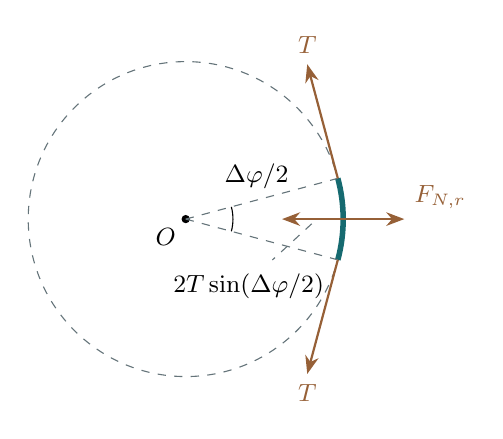
\begin{tikzpicture}
\draw[guide](0,0)circle(2);\fill(0,0)circle(1.5pt)node[below left]{$O$};
\draw[traj,line width=2pt](-15:2)arc(-15:15:2);
\draw[guide](0,0)--(-15:2);\draw[guide](0,0)--(15:2);
\draw[force](15:2)--++(-.388228568,1.448888739)node[above]{$T$};
\draw[force](-15:2)--++(-.388228568,-1.448888739)node[below]{$T$};
\draw[force](2,0)--(2.776457135,0)node[above right]{$F_{N,r}$};
\draw[force](2,0)--(1.223542865,0);
\draw[guide](1.6,-.06)--(1.1,-.52);
\node at(.8,-.85){$2T\sin(\Delta\varphi/2)$};
\draw(.6,0)arc(0:15:.6);\draw(.6,0)arc(0:-15:.6);
\node at(.9,.55){$\Delta\varphi/2$};
\end{tikzpicture}
\figcaption{解图5.1B\quad 有限链弧的俯视图；两端张力沿切线，分布支持力的水平合力须逐段投影。}
\end{minipage}\end{center}
消去 $N$ 和 $\dd\varphi$，得到
\[
 T=\frac{mg}{2\pi}\frac{\cos\beta}{\sin\beta},
\qquad
 \boxed{T=\frac{mg}{2\pi\tan(\alpha/2)}}.
\]
两端张力沿不同切线，其径向分量相加，留下与弧长同阶的向内合力。

\textbf{环半径与锥顶角对张力的影响。}半径 $r$ 约去，是因为同一质量的环越大，单位弧长越轻，同时曲率越小，两者在微元方程中抵消。$\alpha\to0$ 时，锥面接近竖直，支持力的竖直分量很小，所需张力趋于无穷；$\alpha\to\pi$ 时，锥面接近水平，张力趋于零。这些是 $0<\alpha<\pi$ 的锥面接触构型分别趋近两端时的极限。
\subsubsection*{有限弧的张力和支持力}
解图5.1B把短弧画成以正径向为对称轴、两端极角为$\pm\Delta\varphi/2$的有限弧。
令$\lambda=m/(2\pi r)$。在极角$\psi$处，
小段重力为$\lambda gr\,\dd\psi$，竖直平衡给
\[
\dd N\sin\beta=\lambda gr\,\dd\psi.
\]
各段支持力的水平分量沿各处的径向。取有限弧的对称轴为基准，沿轴分量由 $\dd N\cos\beta$ 再乘 $\cos\psi$ 得到。垂直于轴的分量关于对称轴相消：
\[
\begin{aligned}
F_{N,r}
&=\int_{-\Delta\varphi/2}^{\Delta\varphi/2}
\cos\beta\cos\psi\,\dd N\\
&=\lambda gr\cot\beta
\int_{-\Delta\varphi/2}^{\Delta\varphi/2}\cos\psi\,\dd\psi\\
&=2\lambda gr\cot\beta\sin\frac{\Delta\varphi}2.
\end{aligned}
\]
两端张力沿各自切线，其沿对称轴的合力为
$2T\sin(\Delta\varphi/2)$，方向与$F_{N,r}$相反。
取$0<\Delta\varphi<2\pi$，约去非零的正弦因子，仍得
\[
T=\lambda gr\cot\beta=\frac{mg}{2\pi}\cot\beta.
\]
有限弧积分与微元平衡给出同一个张力。取整环时 $\Delta\varphi=2\pi$，两种水平合力都为零，径向合力式成为 $0=0$，张力要由截取的弧段确定。

单位弧长的曲率平衡还可写为
\[
\frac Tr=\lambda g\cot\beta,\qquad
\frac{\dd N}{\dd s}=\frac{\lambda g}{\sin\beta}.
\]
左式中 $T/r$ 是张力方向沿弧改变时产生的向内合力密度。右式是沿锥面外法线的支持力密度，其径向分量为 $(\dd N/\dd s)\cos\beta$。
把$\lambda=m/(2\pi r)$代入才会约去$r$；
若已知的是固定线密度，张力便随环半径增加。
重力加速度$g$没有约去，重力越强、同一几何所需张力越大。
在$0<\beta<\pi/2$时$N,T$均为正，分别符合单侧支持与链条只能受拉的条件。


\Needspace{18\baselineskip}

\pdfbookmark[2]{第 2 题 水平杆靠墙的摩擦条件}{q2}

\section*{第 2 题\quad 水平杆靠墙的摩擦条件}

\tagline{M-05-02}

均匀杆 $AB$ 长为 $l$，重量为 $w_0$。$A$ 端接触粗糙竖直墙，$B$ 端用不可伸长的轻绳悬于墙上的 $C$ 点。杆水平，绳与杆的夹角为 $\theta$，$0<\theta<\pi/2$。
\begin{enumerate}\item 杆与墙的静摩擦系数 $\mu$ 满足什么条件时可以平衡？\item 在距 $A$ 为 $d$ 的位置悬挂重量 $w=w_0/2$ 的重物，$0\le d\le l$。求所需静摩擦系数的最小值与 $d$ 的关系。\end{enumerate}

\begin{center}\begin{minipage}{\linewidth}\centering
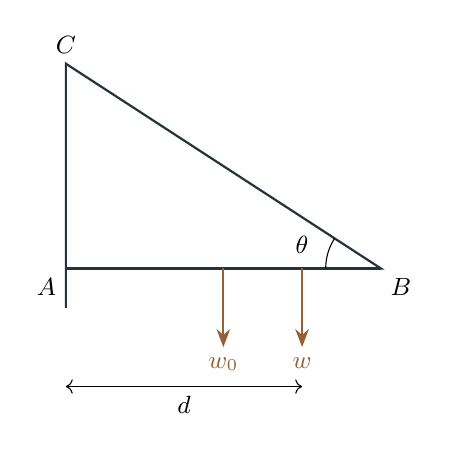
\begin{tikzpicture}
\coordinate(A)at(0,0);\coordinate(B)at(4,0);\coordinate(C)at(0,2.6);\draw[object] (0,-.5)--(C)--(B)--(A);\draw[object] (A)--(B);\draw (3.3,0) arc(180:147:.7);\node at (3.0,.3){$\theta$};\foreach \p/\pos in {A/below left,B/below right,C/above}{\node[\pos]at(\p){$\p$};}\draw[force] (2,0)--(2,-1)node[below]{$w_0$};\draw[force] (3,0)--(3,-1)node[below]{$w$};\draw[<->] (0,-1.5)--(3,-1.5)node[midway,below]{$d$};
\end{tikzpicture}
\figcaption{图 5.2\quad 杆端 $A$ 接触墙，$B$ 端用绳悬于 $C$，挂点距 $A$ 为 $d$。}
\end{minipage}\end{center}

\Needspace{5\baselineskip}\subsection*{解答}

\textbf{墙面摩擦与杆的平衡。}解图5.2A中，墙对杆的法向力 $N$ 水平向右，摩擦力 $f$ 竖直向上，绳张力 $T$ 沿 $BC$ 指向 $C$。静摩擦条件是 $f\le\mu N$，只有临界状态才取等号。
\begin{center}\begin{minipage}{\linewidth}\centering
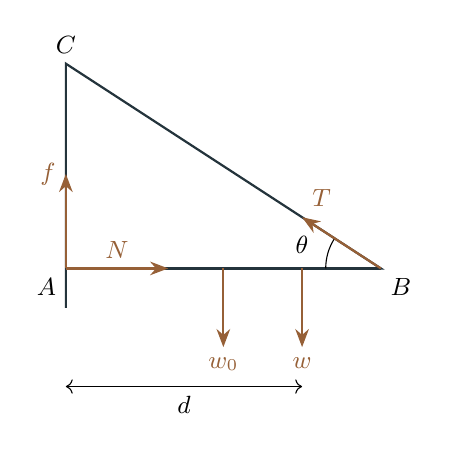
\begin{tikzpicture}
\coordinate(A)at(0,0);\coordinate(B)at(4,0);\coordinate(C)at(0,2.6);\draw[object] (0,-.5)--(C)--(B)--(A);\draw[object] (A)--(B);\draw (3.3,0) arc(180:147:.7);\node at (3.0,.3){$\theta$};\foreach \p/\pos in {A/below left,B/below right,C/above}{\node[\pos]at(\p){$\p$};}\draw[force] (2,0)--(2,-1)node[below]{$w_0$};\draw[force] (3,0)--(3,-1)node[below]{$w$};\draw[<->] (0,-1.5)--(3,-1.5)node[midway,below]{$d$};\draw[force] (0,0)--(0,1.2)node[left]{$f$};\draw[force] (0,0)--(1.3,0)node[midway,above]{$N$};\draw[force] (4,0)--(3, .65)node[above right]{$T$};
\end{tikzpicture}
\figcaption{解图 5.2A\quad 选 $B$ 为力矩中心可消去绳张力；重物在杆内时，墙上摩擦向上。}
\end{minipage}\end{center}
水平、竖直平衡分别为
\begin{align*}
 N&=T\cos\theta,\\
 f+T\sin\theta&=w_0+w.
\end{align*}
对 $B$ 取矩，绳张力的力矩为零。$N$ 的作用线沿杆，也没有力矩。摩擦力与两个重力的力矩相抵：
\[
 fl=\frac{w_0l}{2}+w(l-d).
\]
因而
\[
 f=\frac{w_0}{2}+w\left(1-\frac dl\right),
 \qquad T\sin\theta=\frac{w_0}{2}+\frac{wd}{l},
 \qquad N=\left(\frac{w_0}{2}+\frac{wd}{l}\right)\cot\theta.
\]
当 $0\le d\le l$、$w\ge0$ 时，$f>0,N>0$，与图中的方向一致。

\textbf{第一问：不挂附加重物。}令 $w=0$，则 $f=w_0/2$，$N=(w_0/2)\cot\theta$，故
\[
 \boxed{\mu\ge\tan\theta}.
\]
所需摩擦力由平衡方程给出，在最小系数处恰达到最大静摩擦力 $f=\mu N$。

\textbf{第二问：附加重物为杆重的一半。}令 $w=w_0/2$，得到
\[
 f=\frac{w_0}{2}\left(2-\frac dl\right),
 \qquad N=\frac{w_0}{2}\left(1+\frac dl\right)\cot\theta.
\]
于是
\[
 \boxed{\mu_{\min}(d)=\frac{2l-d}{l+d}\tan\theta},
 \qquad 0\le d\le l.
\]
其导数为
\[
 \frac{\dd\mu_{\min}}{\dd d}
 =-\frac{3l\tan\theta}{(l+d)^2}<0.
\]
把重物从 $A$ 移向 $B$，所需摩擦力减小而法向力增大，所以所需摩擦系数单调减小。三个位置为
\[
 d=0:\ 2\tan\theta;\qquad
 d=l/2:\ \tan\theta;\qquad
 d=l:\ \tfrac12\tan\theta.
\]
给定墙面材料的$\mu$后，还可直接从结果读允许的挂重位置。记$c=\mu/\tan\theta$，静止条件为
\[c\ge\frac{2-d/l}{1+d/l}
\quad\Longrightarrow\quad \frac dl\ge\frac{2-c}{1+c}.\]
若 $c<1/2$，杆上没有可用挂点。若 $1/2\le c<2$，从 $d=l(2-c)/(1+c)$ 到右端点 $B$ 都可挂重物。若 $c\ge2$，整段 $0\le d\le l$ 都允许。解图5.2A中把重物向绳连接端移动，同时减小墙所需向上摩擦、增加绳张力的水平压紧分量，所以这两个作用共同降低摩擦系数要求。

对$A$取矩时，墙端两力作用于矩心，力矩为零。方程$Tl\sin\theta=w_0l/2+wd$先给出$T$，再由竖直平衡得到相同的$f$。
\subsubsection*{用图读挂点范围与摩擦余量}
令$x=d/l$、$c=\mu/\tan\theta$，解图5.2B画出所需系数
$c_{\min}(x)=(2-x)/(1+x)$。给定材料时$c$是水平线；
曲线给出各挂点所需的最小系数。给定挂点 $x$，材料线在该点的纵坐标满足 $c\ge c_{\min}(x)$ 时，杆能保持静止。
\begin{center}\begin{minipage}{\linewidth}\centering
\begin{tikzpicture}[x=5cm,y=1.6cm]
\draw[axis](0,0)--(1.18,0)node[right]{$x=d/l$};
\draw[axis](0,0)--(0,2.35)node[above]{$c=\mu/\tan\theta$};
\fill[accent!12](2/3,.8)--(1,.8)--(1,.5)
plot[domain=1:2/3,samples=40](\x,{(2-\x)/(1+\x)})--cycle;
\draw[traj,domain=0:1,samples=90]plot(\x,{(2-\x)/(1+\x)});
\draw[warm](0,.8)--(1.05,.8)node[right]{$c=0.8$};
\draw[guide](2/3,0)--(2/3,.8);
\foreach \x/\y/\lab in {0/2/{2},.5/1/{1},1/.5/{1/2}}
{\fill(\x,\y)circle(1.6pt);\node[above right]at(\x,\y){$\lab$};}
\node[below]at(.5,0){$1/2$};\node[below]at(2/3,0){$2/3$};\node[below]at(1,0){$1$};
\draw[<->,accent](2/3,.18)--(1,.18)node[midway,above]{允许挂点};
\end{tikzpicture}
\figcaption{解图5.2B\quad 材料示例$\mu=0.8\tan\theta$；阴影是供给上限与所需系数之差，须有$d/l\geq2/3$。}
\end{minipage}\end{center}
图中$x=1/2$给$c_{\min}=1$。
附加重物挂在杆中点时，它与杆重有同一作用线，
两者合起来相当于重量增大而作用点不动；
所需$f,N$都成为无附加重物时的$3/2$倍，所以比值仍是$\tan\theta$。


\subsubsection*{附加重量越大，摩擦条件一定越苛刻吗}
保留任意$w\geq0$，两平衡力给
\[
\mu_{\min}(x,w)
=\frac{w_0/2+w(1-x)}{w_0/2+wx}\tan\theta.
\]
固定挂点$x$，对$w$求导：
\[
\frac{\partial\mu_{\min}}{\partial w}
=\frac{(w_0/2)(1-2x)}{(w_0/2+wx)^2}\tan\theta.
\]
因此挂点在左半杆时，加重使所需系数增大；
在右半杆时，加重反而使所需系数减小；
恰在中点时系数与$w$无关。
挂点在右半杆时，增加重物使墙压增大得比所需摩擦快，因而比值下降。挂在最右端时，摩擦大小保持不变，墙压仍随重物增加。
这一区分需要同时保留$f$与$N$，只比较总重量或一个力矩看不出结果。

摩擦系数的下限由 $f/N$ 决定。绳和墙各自的负荷仍要由张力 $T$ 和墙压 $N$ 表示，绳张力为
\[
T=\frac{w_0/2+wx}{\sin\theta}.
\]
当$\theta$变小时，所需摩擦系数随$\tan\theta$减小，
但$T$及墙压$N=T\cos\theta$反而增大。
减小绳角会使防滑更容易，同时增大绳和墙承担的力。


\Needspace{18\baselineskip}

\pdfbookmark[2]{第 3 题 竖杆受水平力的防滑条件}{q3}

\section*{第 3 题\quad 竖杆受水平力的防滑条件}

\tagline{M-05-03}

质量为 $m$、长为 $L$ 的均匀细杆竖直放置，下端接触水平地面，静摩擦系数为 $\mu$。上端由轻绳拉住，绳的另一端固定在左下方，绳与竖杆的夹角为 $\theta$，$0<\theta<\pi/2$。在离地高度 $h$ 处向右施加水平力 $F$，$0\le h\le L$。求保持杆不滑倒所允许的 $F$ 的最大值，并讨论何时仅凭摩擦条件不能给出有限上限。

\begin{center}\begin{minipage}{\linewidth}\centering
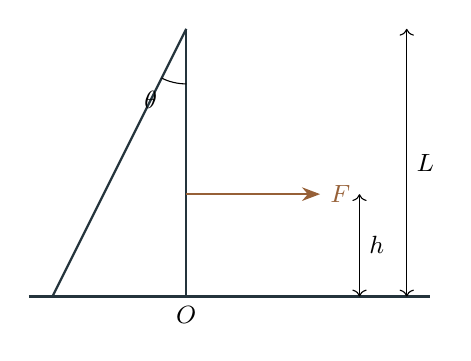
\begin{tikzpicture}
\draw[object](-2,0)--(3.1,0);
\draw[object](0,0)--(0,3.4);\draw[object](-1.7,0)--(0,3.4);
\draw(0,2.7)arc(-90:-116.565051177:.7);\node at(-.45,2.5){$\theta$};
\draw[force](0,1.3)--(1.7,1.3)node[right]{$F$};
\draw[<->](2.2,0)--(2.2,1.3)node[midway,right]{$h$};
\draw[<->](2.8,0)--(2.8,3.4)node[midway,right]{$L$};
\node[below]at(0,0){$O$};
\end{tikzpicture}
\figcaption{图5.3\quad 绳固定在左下方，推力高度$h$与杆长$L$分别标出。}\end{minipage}\end{center}

\Needspace{5\baselineskip}\subsection*{解答}

\textbf{力的方向。}解图5.3A中，绳张力的水平分量向左、竖直分量向下；地面摩擦 $f$ 向左，支持力 $N$ 向上。由于杆保持竖直，重力通过下端 $O$，对 $O$ 不产生力矩。
\begin{center}\begin{minipage}{\linewidth}\centering
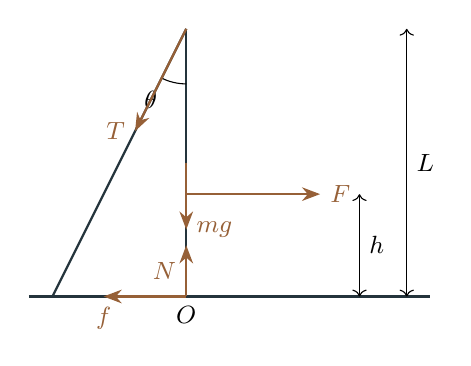
\begin{tikzpicture}
\draw[object](-2,0)--(3.1,0);
\draw[object](0,0)--(0,3.4);\draw[object](-1.7,0)--(0,3.4);
\draw(0,2.7)arc(-90:-116.565051177:.7);\node at(-.45,2.5){$\theta$};
\draw[force](0,1.3)--(1.7,1.3)node[right]{$F$};
\draw[<->](2.2,0)--(2.2,1.3)node[midway,right]{$h$};
\draw[<->](2.8,0)--(2.8,3.4)node[midway,right]{$L$};
\node[below]at(0,0){$O$};
\draw[force](0,3.4)--(-.65,2.1)node[left]{$T$};
\draw[force](0,0)--(-1.05,0)node[below]{$f$};
\draw[force](0,0)--(0,.65)node[midway,left]{$N$};
\draw[force](0,1.7)--(0,.85)node[right]{$mg$};
\end{tikzpicture}
\figcaption{解图5.3A\quad 地面摩擦向左，绳向下压紧；箭头标各力实际作用点和方向，大小由平衡方程确定。}\end{minipage}\end{center}
对 $O$ 取矩，并列水平、竖直平衡：
\begin{align*}
 TL\sin\theta&=Fh,\\
 T\sin\theta+f&=F,\\
 N&=mg+T\cos\theta.
\end{align*}
故
\[
 T=\frac{Fh}{L\sin\theta},\qquad
 f=F\left(1-\frac hL\right),\qquad
 N=mg+\frac{Fh}{L}\cot\theta.
\]
$0\le h\le L$ 时 $f\ge0$，所假定的向左方向成立。若改对杆上端取矩，直接得到 $fL=F(L-h)$，也得到相同的摩擦力。

\textbf{地面摩擦与推力范围。}不滑动要求
\[
 F\left(1-\frac hL\right)
 \le\mu\left(mg+\frac{Fh}{L}\cot\theta\right),
\]
即
\[
 DF\le\mu mgL,\qquad
 D=L-h-\mu h\cot\theta.
\]
\begin{enumerate}
\item 若 $D>0$，才可除以 $D$ 而不改变不等号方向，得到有限上限
\[
 \boxed{F_{\max}=\frac{\mu mgL}{L-h-\mu h\cot\theta}
 =\frac{\mu mgL\tan\theta}{(L-h)\tan\theta-\mu h}}.
\]
此时 $h<L\tan\theta/(\mu+\tan\theta)$。
\item 若 $D\le0$，左端对任意 $F\ge0$ 均不为正，而右端不为负，摩擦条件始终满足。在理想刚杆、无限强度绳的模型中，$F$ 没有有限上限。绳的强度若有给定上限，再用张力式与该上限联立。
\end{enumerate}
\begin{center}\begin{minipage}{\linewidth}\centering
\begin{tikzpicture}[x=5.5cm,y=.9cm]
\fill[accent!8](.5,0)rectangle(1,4.35);
\draw[axis](0,0)--(1.14,0)node[right]{$h/L$};
\draw[axis](0,0)--(0,4.8)node[above]{$F_{\max}/mg$};
\draw[guide](.5,0)--(.5,4.4);
\draw[traj,domain=0:.44,samples=90]plot(\x,{.5/(1-2*\x)});
\foreach \x/\lab in {0/0,.25/{1/4},.5/{1/2},.75/{3/4},1/1}
{\draw(\x,-.06)--(\x,.06);\node[below]at(\x,-.1){$\lab$};}
\foreach \y in {1,2,3,4}{\draw(-.01,\y)--(.01,\y);\node[left]at(-.01,\y){$\y$};}
\node[left]at(0,.5){$\mu=1/2$};
\node[align=center]at(.77,2.7){摩擦条件\\不设有限上限};
\end{tikzpicture}
\figcaption{解图5.3B\quad 参数示例$\mu=1/2,\cot\theta=2$；$h/L<1/2$有有限上限，从 $h/L=1/2$ 起，摩擦条件对任意非负推力都成立。}
\end{minipage}\end{center}
\textbf{施力高度与两端情形。}解图5.3B中，在有限上限区，$D$ 随 $h$ 减小，因而 $F_{\max}$ 随 $h$ 增大。施力越高，绳承担的水平分力越多，地面所需摩擦越少；绳的向下分量同时增大 $N$。

$h=0$ 时绳不需张力，$F_{\max}=\mu mg$；$h=L$ 时 $f=0$，绳承担全部水平力，摩擦不限制 $F$。若 $\mu=0$，则除 $h=L$ 外只能有 $F=0$。这些结论也由未经除法的原始不等式直接得到。
\subsubsection*{从摩擦比的增长率解释无有限上限}
令$x=h/L$。在给定作用高度下，所需摩擦与地面支持力之比为
\[
\frac fN=\frac{(1-x)F}{mg+xF\cot\theta}.
\]
对$0\leq x<1$，它随$F$增加而增加：
\[
\frac{\partial(f/N)}{\partial F}
=\frac{(1-x)mg}{(mg+xF\cot\theta)^2}>0.
\]
$x=0$时这个比值没有上界，恢复$F\leq\mu mg$。
对$0<x<1$，其极限却是有限的
\[
\lim_{F\to\infty}\frac fN
=\frac{1-x}{x}\tan\theta.
\]
若材料的$\mu$不小于这个极限，就不会与增长中的$f/N$发生交叉，
所以理想静摩擦条件不能给有限最大推力。
将该条件整理，正是$x\geq\tan\theta/(\mu+\tan\theta)$。
当 $\mu>0$、$D=0$ 时，法向力仍含正的常量 $mg$，因而每个有限的 $F$ 都有 $f<\mu N$。只有在 $F\to\infty$ 的极限，所需的摩擦比才趋于 $\mu$。

有限上限区中还可直接求导：
\[
\frac{\dd F_{\max}}{\dd h}
=\frac{\mu mgL(1+\mu\cot\theta)}
{(L-h-\mu h\cot\theta)^2}>0\quad(\mu>0).
\]
解图5.3B采用$\mu=1/2,\cot\theta=2$的一组参数，
渐近线确在$h/L=1/2$，曲线为$F_{\max}/mg=(1/2)/(1-2h/L)$。
图中横坐标使用实际无量纲高度，渐近线右侧仍属于$0\leq h/L\leq1$的允许几何，
表示任意非负推力都满足静摩擦条件。

若固定$F>0$反求高度，未经除法的不等式给
\[
\frac hL\geq
\frac{1-\mu mg/F}{1+\mu\cot\theta}.
\]
当$F\leq\mu mg$，右端非正，任意高度均可；
当$F>\mu mg$，须把施力点提高到所给下界。
这一结论与$F_{\max}$随高度增大的曲线相符。


\Needspace{18\baselineskip}

\pdfbookmark[2]{第 4 题 半球凹面内的均匀细杆}{q4}

\section*{第 4 题\quad 半球凹面内的均匀细杆}

\tagline{M-05-04}

半径为 $R$ 的光滑半球形凹面内，一根刚性均匀细杆处于平衡。杆的一端接触内壁，杆身经过凹面边缘并伸出，如图所示。已知杆在凹面内的部分长为 $l$，求露出部分的长度，并给出该接触构型的适用范围。

\begin{center}\begin{minipage}{\linewidth}\centering
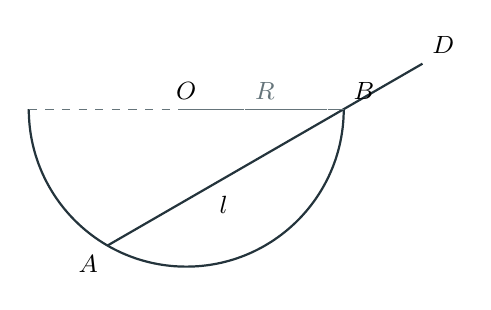
\begin{tikzpicture}
\coordinate(O)at(0,0);\coordinate(A)at(-1,-1.732050808);
\coordinate(B)at(2,0);\coordinate(D)at(3,.577350269);
\draw[object](-2,0)arc(180:360:2);\draw[guide](-2,0)--(2,0);
\draw[object](A)--(D);\draw[guide](O)--(B)node[midway,above]{$R$};
\node[above]at(O){$O$};\node[below left]at(A){$A$};
\node[above right]at(B){$B$};\node[above right]at(D){$D$};
\node[below right]at(.3,-.98){$l$};
\end{tikzpicture}
\figcaption{图5.4\quad 杆内端$A$接触凹面，杆身在边缘$B$处支承并伸出至$D$。}\end{minipage}\end{center}

\Needspace{5\baselineskip}\subsection*{解答}

\textbf{利用三力共点确定整杆重心。}设杆内端为 $A$，凹面边缘的接触点为 $B$，外端为 $D$，球心为 $O$，整杆重心为 $C$。光滑球面对 $A$ 的支持力沿 $AO$；边缘对细杆的支持力垂直杆。两条作用线交于 $E$。三个非平行力平衡，重力作用线也经过 $E$，因此 $EC$ 竖直。
\begin{center}\begin{minipage}{\linewidth}\centering
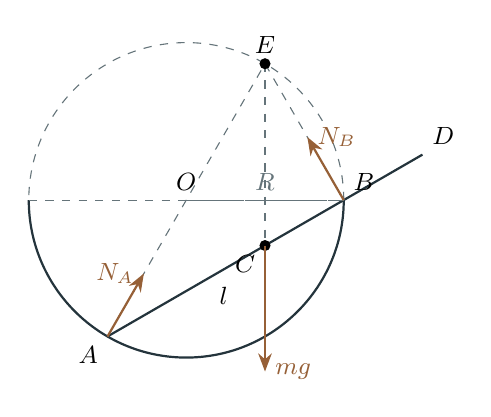
\begin{tikzpicture}
\coordinate(O)at(0,0);\coordinate(A)at(-1,-1.732050808);
\coordinate(B)at(2,0);\coordinate(D)at(3,.577350269);
\draw[object](-2,0)arc(180:360:2);\draw[guide](-2,0)--(2,0);
\draw[object](A)--(D);\draw[guide](O)--(B)node[midway,above]{$R$};
\node[above]at(O){$O$};\node[below left]at(A){$A$};
\node[above right]at(B){$B$};\node[above right]at(D){$D$};
\node[below right]at(.3,-.98){$l$};
\draw[guide](2,0)arc(0:180:2);
\coordinate(E)at(1,1.732050808);\coordinate(C)at(1,-.577350269);
\draw[guide](A)--(E)--(B);\draw[guide](E)--(C);
\fill(E)circle(2pt)node[above]{$E$};\fill(C)circle(2pt)node[below left]{$C$};
\draw[force](A)--(-.538119785,-.932050808)node[left]{$N_A$};
\draw[force](B)--(1.538119785,.8)node[right]{$N_B$};
\draw[force](C)--(1,-2.177350269)node[right]{$mg$};
\end{tikzpicture}
\figcaption{解图5.4A\quad 上半虚圆为辅助圆，$AE$为直径；$C$是整杆中点，三力作用线共点。}\end{minipage}\end{center}
在解图5.4A中，延长 $AO$ 到球面的另一交点 $E$。因 $AE$ 为直径、$B$ 在球面上，圆周角给出 $\angle ABE=90^\circ$，正好满足边缘法向力垂直杆。因此
\[
 AE=2R,\qquad AB=l,\qquad BE^2=4R^2-l^2.
\]
令杆与水平面的夹角为 $\gamma$。直角三角形 $ABE$ 中 $BE/l=\tan\gamma$，而 $EC$ 竖直，在三角形 $BCE$ 中 $CB/BE=\tan\gamma$。所以
\[
 CB=BE\tan\gamma=\frac{BE^2}{AB}
 =\frac{4R^2-l^2}{l}.
\]
\textbf{重心在整根杆的中点。}图中 $C$ 位于 $A,B$ 之间，$AC=l-CB$，均匀杆满足 $CD=AC$。于是露出长度
\begin{align*}
 BD&=CD-CB=AC-CB=l-2CB\\
 &=l-2\frac{4R^2-l^2}{l}
 =\boxed{\frac{3l^2-8R^2}{l}}.
\end{align*}
\begin{center}\begin{minipage}{\linewidth}\centering
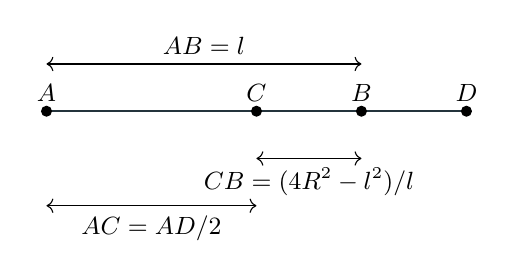
\begin{tikzpicture}
\coordinate(A)at(0,0);\coordinate(B)at(4,0);
\coordinate(D)at(5.333333333,0);\coordinate(C)at(2.666666667,0);
\draw[object](A)--(D);
\draw[<->](0,.6)--(4,.6)node[midway,above]{$AB=l$};
\draw[<->](2.666666667,-.6)--(4,-.6)node[midway,below]{$CB=(4R^2-l^2)/l$};
\draw[<->](0,-1.2)--(2.666666667,-1.2)node[midway,below]{$AC=AD/2$};
\foreach \p in {A,B,C,D}{\fill(\p)circle(2pt);\node[above]at(\p){$\p$};}
\end{tikzpicture}
\figcaption{解图5.4B\quad 与解图5.4A同一长度比例的展平图；$C$分的是整杆$AD$。}
\end{minipage}\end{center}
重力作用于整根杆$AD$的中点$C$。解图5.4B把$AC=AD/2$和$AB=l$分别标出。

\textbf{接触构型的范围。}弦长给出 $l\le2R$，且 $BD\ge0$ 要求
\[
 l\ge\sqrt{\frac83}\,R.
\]
若有实际露出部分并保持两个非退化接触，则
\[
 \boxed{\sqrt{8/3}\,R<l<2R}.
\]
长度取下限时 $BD=0$，外端恰在口缘。长度接近上限时，杆趋于水平，内端支持力趋于零。

几何关系 $l=2R\cos\gamma$ 给出 $0<\gamma\le35.264^\circ$。设整杆质量为 $m$，在这一角度范围内，将两个支持力分别沿水平和竖直方向投影，得到
\[
 N_A=mg\tan\gamma,\qquad
 N_B=mg\frac{\cos2\gamma}{\cos\gamma}.
\]
此范围两者均非负，故几何与单向接触条件一致。
\subsubsection*{由坐标求重心线和露出长度}
为明确两次倾角关系，在三角形$AOB$中$OA=OB=R$，
$\angle ABO=\gamma$，所以$\angle OAB=\gamma$；
$A,O,E$共线，故直角三角形$ABE$中的$\angle BAE$也为$\gamma$。
由直角三角形 $ABE$ 得 $BE/AB=\tan\gamma$。解图5.4A 的上半圆是延长后的辅助截面圆，$E$ 是两条支持力作用线的交点，实际接触点为 $A,B$。

也可令$B=(R,0)$，杆沿外伸方向的单位向量为
$\vect t=(\cos\gamma,\sin\gamma)$，整杆长为$s=AD$。
于是
\[
A=B-l\vect t,\qquad |OA|=R
\quad\Longrightarrow\quad l=2R\cos\gamma.
\]
支持力交点为$E=-A$，整杆中点$C=A+(s/2)\vect t$。
由重心线竖直，$C_x=E_x$：
\[
R-l\cos\gamma+\frac s2\cos\gamma
=-R+l\cos\gamma,
\]
\[
s=4l-\frac{4R}{\cos\gamma}
=4l-\frac{8R^2}{l},\qquad
BD=s-l=\frac{3l^2-8R^2}{l}.
\]
坐标式把弦长、整杆中点和三力共点连在一起。解图5.4A 中的 $C$ 与解图5.4B 的展开图对应，都是整个 $AD$ 的中点。两图取 $\gamma=30^\circ$、$l=2\sqrt3$、$R=2$，代入露出长度式得 $BD=2/\sqrt3$。

\subsubsection*{露出段消失和内端支持力消失}
在$A$，法向力方向与水平线夹角为$2\gamma$；
在$B$，法向力方向为$(-\sin\gamma,\cos\gamma)$。
水平和竖直分量方程为
\[
N_A\cos2\gamma-N_B\sin\gamma=0,\qquad
N_A\sin2\gamma+N_B\cos\gamma=mg.
\]
消元恢复$N_A=mg\tan\gamma$、$N_B=mg\cos2\gamma/\cos\gamma$，
因而不仅作用线共点，两支持力也都能以非负大小实现平衡。
在露出段刚为零的下界，$\cos\gamma=\sqrt{2/3}$，
\[
N_A=\frac{mg}{\sqrt2},\qquad N_B=\frac{mg}{\sqrt6},
\]
两者都没有消失，退化的是$BD$的长度。
在$l\to2R$的上界，$\gamma\to0$，才有$N_A\to0$、$N_B\to mg$；
此时$C$趋向边缘$B$，三力非平行的普通构型也随之退化。
下端先使露出段消失，上端则使内端支持力消失，分别对应上述两组极限。


\Needspace{18\baselineskip}

\pdfbookmark[2]{第 5 题 三圆柱堆放的摩擦下限}{q5}

\section*{第 5 题\quad 三圆柱堆放的摩擦下限}

\tagline{M-05-05}

三个半径和质量均相同的圆柱体互相接触，在水平地面上堆成两下、上一的对称构型。圆柱之间的静摩擦系数为 $\mu_1$，圆柱与地面之间为 $\mu_2$。求使三个圆柱静止所需的 $\mu_1$ 和 $\mu_2$ 的下限。

\begin{center}\begin{minipage}{\linewidth}\centering
\begin{tikzpicture}
\draw[object] (-2.4,0)--(2.4,0);\foreach \x/\y/\s in {-1/1/B,1/1/C,0/2.732/A}{\draw[object] (\x,\y)circle(1);\fill(\x,\y)circle(1.5pt);\node at(\x,\y+.25){$\s$};}\draw[guide] (-1,1)--(1,1)--(0,2.732)--cycle;\node[right]at(2,1.7){$r,m$ 相同};
\end{tikzpicture}
\figcaption{图 5.5\quad 三圆柱两两相切，圆心围成等边三角形。}
\end{minipage}\end{center}

\Needspace{5\baselineskip}\subsection*{解答}

\textbf{上柱与下柱的隔离受力。}设每柱质量为 $m$。上柱与每个下柱之间的法向力为 $N$、摩擦力为 $f$；每个下柱受地面支持力 $N_2$、向内的摩擦力 $f_2$。保留下层两柱之间的法向力 $Q$。镜面对称使这个竖直接触面的切向力为零，但法向力仍可以存在。
\begin{center}\begin{minipage}{\linewidth}\centering
\begin{tikzpicture}
\draw[object](0,0)circle(1);
\draw[force](-.5,-.866025404)--(.05,.086602540)node[above right]{$N$};
\draw[force](.5,-.866025404)--(-.05,.086602540)node[above left]{$N$};
\draw[force](-.5,-.866025404)--(-.755255888,-.718653348)node[above left]{$f$};
\draw[force](.5,-.866025404)--(.755255888,-.718653348)node[above right]{$f$};
\draw[force](0,0)--(0,-2.2)node[below]{$mg$};
\node at(0,1.45){上圆柱};
\end{tikzpicture}
\figcaption{解图5.5A\quad 以最低摩擦状态的大小比例绘受力；两侧法向力和摩擦的水平分量分别相消。}
\end{minipage}\end{center}
解图5.5A把上柱单独隔离，两个接触点的法线均沿圆心连线；解图5.5B再隔离一个下柱，保留它与另一根下柱之间的水平推力$Q$。这两张图使用同一对作用与反作用，因而柱间摩擦$f$在两柱上的方向相反；下柱绕自身圆心取矩时，法向力不贡献力矩，才能把地面摩擦$f_2$与$f$联系起来。

圆心连线与水平成 $60^\circ$，上柱两侧法向力均斜向内、向上，摩擦力斜向外、向上。上柱竖直平衡为
\[
 2N\sin60^\circ+2f\cos60^\circ=mg,
 \qquad \sqrt3N+f=mg.\tag{1}
\]
两侧水平分量和力矩因对称抵消。
\begin{center}\begin{minipage}{\linewidth}\centering
\begin{tikzpicture}
\draw[object](0,1)circle(1);\draw[object](-1.5,0)--(1.6,0);
\draw[force](-.5,1.866025404)--(.05,.913397460)node[below right]{$N$};
\draw[force](-.5,1.866025404)--(-.755255888,1.718653348)node[above left]{$f$};
\fill(-1,1)circle(1.5pt);\draw[guide](-1,1)--(-1.65,1.45);
\node[above left]at(-1.65,1.45){$Q=0$（临界）};
\draw[force](0,0)--(-.294744112,0)node[below left]{$f_2$};
\draw[force](0,0)--(0,3.3)node[above right]{$N_2$};
\draw[force](0,1)--(0,-1.2)node[below]{$mg$};
\node at(2.6,1.5){右下圆柱};
\end{tikzpicture}
\figcaption{解图5.5B\quad 最低摩擦临界状态取$Q=0$；一般平衡仍保留$Q\geq0$，各实际作用点用于圆心矩。}
\end{minipage}\end{center}
\textbf{下柱还须满足转动平衡。}取右下柱。地面法向力、重力、圆柱间法向力都通过圆心，不产生力矩；上接触摩擦与地面摩擦有相等力臂 $r$，转向相反，故
\[
 rf-rf_2=0,\qquad f_2=f.\tag{2}
\]
竖直、水平平衡分别是
\begin{align*}
 N_2&=mg+N\sin60^\circ+f\cos60^\circ=\frac32mg,\tag{3}\\
 \frac N2-\frac{\sqrt3}2f+Q-f_2&=0.\tag{4}
\end{align*}
从(1)、(2)、(4)得到
\[
 N=\frac{mg-f}{\sqrt3},\qquad
 Q=\frac{(4+2\sqrt3)f-mg}{2\sqrt3}.
\]
下层两柱之间是单侧接触，法向力取$Q\ge0$，因此
\[
 f\ge f_*:=\frac{mg}{4+2\sqrt3}
 =\frac{2-\sqrt3}{2}mg.
\]
$f$的最小值使$Q$恰为零，两下柱此时保持几何相切。

\textbf{两个摩擦下限同时取到。}在 $0\le f<mg$ 内，$N>0$，所需比值
\[
 \frac fN=\frac{\sqrt3 f}{mg-f},\qquad
 \frac{f_2}{N_2}=\frac{2f}{3mg}
\]
都随 $f$ 增大。因此使两个摩擦系数最小的构型是 $f=f_*$、$Q=0$。由(1)得 $N=mg/2$，从而
\[
 \boxed{\mu_1\ge2-\sqrt3},\qquad
 \boxed{\mu_2\ge\frac{2-\sqrt3}{3}}.
\]
数值约为 $0.26795$ 和 $0.08932$。这两个条件不仅必要，而且充分：取上述 $N,f,N_2,f_2,Q$，所有平衡方程都成立，且各接触力均非负、各摩擦力均不超限。地面摩擦大小虽与柱间摩擦相同，支持力却是三倍，所以两种摩擦系数下限不能相等。
\subsubsection*{为什么可以在对称受力中求下限}
若已有一组可行接触力，将它关于竖直中线镜像，就得到另一组可行解。
两组的平均也满足每根圆柱的合力、力矩方程。
对同一接触，库仑约束$|f|\leq\mu N$及$N\geq0$构成凸集合，
所以平均后的接触力仍满足各摩擦上限与单侧接触。
这组平均解左右对称，下层两柱接触处的竖直切向力与其镜像相反，平均为零，
水平法向力$Q$则保留。
因此使用对称方程没有排除任何“存在平衡”的材料参数，所求下限仍是完整下限。

\subsubsection*{给定两种材料时的对称接触力}
前面以$f$参数化平衡力，两个摩擦不等式分别给
\[
\frac{\sqrt3 f}{mg-f}\leq\mu_1
\quad\Longrightarrow\quad
f\leq\frac{\mu_1mg}{\sqrt3+\mu_1},
\]
\[
\frac{2f}{3mg}\leq\mu_2
\quad\Longrightarrow\quad
f\leq\frac32\mu_2mg.
\]
结合$Q\geq0$，可行区间为
\[
\boxed{\frac{mg}{4+2\sqrt3}\leq f\leq
\min\left(\frac{\mu_1mg}{\sqrt3+\mu_1},\frac32\mu_2mg\right)}.
\]
只要此区间非空，代回$N=(mg-f)/\sqrt3$、$N_2=3mg/2$、
$f_2=f$和$Q$的表达式，就能构造完整静力解。
区间非空的条件恰为两个系数分别不小于前述下限。
提高地面摩擦系数不能补偿不足的柱间系数，反之亦然；
两个约束限制的是同一$f$的不同上界。

在最低系数的临界状态，
\[
N=\frac{mg}{2},\quad f=f_2=\frac{2-\sqrt3}{2}mg,\quad
N_2=\frac{3mg}{2},\quad Q=0.
\]
在摩擦系数取下限时，下层两柱刚好相切，接触法向力 $Q=0$。
当材料系数更大时，静摩擦只需落在可行区间，不必把每个接触都取成$f=\mu N$。


\Needspace{18\baselineskip}

\pdfbookmark[2]{第 6 题 斜木板上三球的支承}{q6}

\section*{第 6 题\quad 斜木板上三球的支承}

\tagline{M-05-06}

均匀木板 $AB$ 长 $L=100\,\mathrm{cm}$，重 $2G$。$A$ 端铰接在竖直墙上，$B$ 端由水平轻绳拉住，木板与墙的夹角为 $60^\circ$。三个相同小球沿木板排列，彼此接触且都接触木板；最左球还接触墙。每球半径 $R=10\,\mathrm{cm}$，重 $G$。球与墙、木板以及球之间均光滑。求水平绳的张力 $T$。

\begin{center}\begin{minipage}{\linewidth}\centering
\begin{tikzpicture}
\coordinate(A)at(0,0);\coordinate(B)at(5.196152423,3);
\coordinate(E)at(.9,.519615242);\coordinate(F)at(1.939230485,1.119615242);
\coordinate(K)at(2.978460969,1.719615242);\coordinate(D)at(1.679422863,.969615242);
\draw[object](0,-.3)--(0,3.5);\draw[object](A)--(B)--(0,3);
\foreach \x/\y in {.6/1.039230485,1.639230485/1.639230485,2.678460969/2.239230485}
{\draw[object](\x,\y)circle(.6);}
\draw(0,.7)arc(90:30:.7);\node at(.45,.78){$60^\circ$};
\node[below]at(A){$A$};\node[right]at(B){$B$};
\node[above]at(3.7,3){水平绳};\node[below right]at(3.7,1.9){$L=10R$};
\end{tikzpicture}
\figcaption{图5.6\quad 三球与板、墙接触；木板长度及球半径按$L:R=10:1$绘制。}
\end{minipage}\end{center}

\Needspace{5\baselineskip}\subsection*{解答}

\textbf{先研究三个球组成的整体。}板与水平成 $\beta=30^\circ$。整体重力 $3G$ 通过中球中心 $C$；墙对左球的支持力 $N_1$ 水平向右；木板对三球的法向力合为 $N_2$，垂直木板。球间接触力都是内力。
\begin{center}\begin{minipage}{\linewidth}\centering
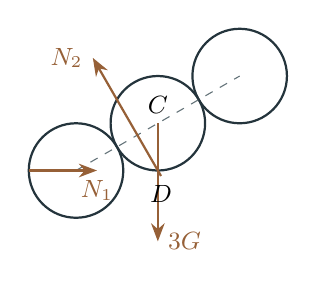
\begin{tikzpicture}
\coordinate(A)at(0,0);\coordinate(B)at(5.196152423,3);
\coordinate(E)at(.9,.519615242);\coordinate(F)at(1.939230485,1.119615242);
\coordinate(K)at(2.978460969,1.719615242);\coordinate(D)at(1.679422863,.969615242);
\foreach \x/\y in {.6/1.039230485,1.639230485/1.639230485,2.678460969/2.239230485}
{\draw[object](\x,\y)circle(.6);}
\draw[guide](.6,1.039230485)--(2.678460969,2.239230485);
\draw[force](0,1.039230485)--(.866025404,1.039230485)node[below]{$N_1$};
\draw[force](D)--(.813397459,2.469615242)node[left]{$N_2$};
\draw[force](1.639230485,1.639230485)--(1.639230485,.139230485)node[right]{$3G$};
\node[above]at(1.639230485,1.639230485){$C$};\node[below]at(D){$D$};
\end{tikzpicture}
\figcaption{解图5.6A\quad 墙力对$C$逆时针，板合力对$C$顺时针；$D$在中球垂足左侧。}
\end{minipage}\end{center}
解图5.6A将三球作为整体，其竖直、水平平衡给出
\[
 N_2\cos30^\circ=3G,\qquad
 N_1=N_2\sin30^\circ,
\]
所以 $N_2=2\sqrt3G$，$N_1=\sqrt3G$。

\textbf{求板上合力的作用点。}设左球中心在板上的垂足为 $E$，中球中心的垂足为 $F$，合力作用点为 $D$。由于三球都接触板，相邻圆心距为 $2R$，$EF=2R$。墙与板夹角为 $60^\circ$，左球中心在该夹角的角平分线上，故
\[
 AE=R\cot30^\circ=\sqrt3R.
\]
墙力的作用线通过左球中心；它到 $C$ 的竖直距离为 $2R\sin30^\circ=R$。对整体关于$C$取矩，$N_1$向右且作用线在$C$下方，产生逆时针力矩；板合力作用点在$F$左侧时产生顺时针力矩，二者相抵。令 $FD=x$，则
\[
 N_2x=N_1R,\qquad x=\frac R2.
\]
因此
\[
 AD=AE+EF-FD=\left(\sqrt3+\frac32\right)R.
\]
\textbf{再研究木板。}解图5.6B中，球给木板的压力大小为 $N_2$、方向垂直板向下右，作用于 $D$。板重 $2G$ 作用于中点。铰链可同时提供 $A_x,A_y$，对 $A$ 取矩可一并消去。
\begin{center}\begin{minipage}{\linewidth}\centering
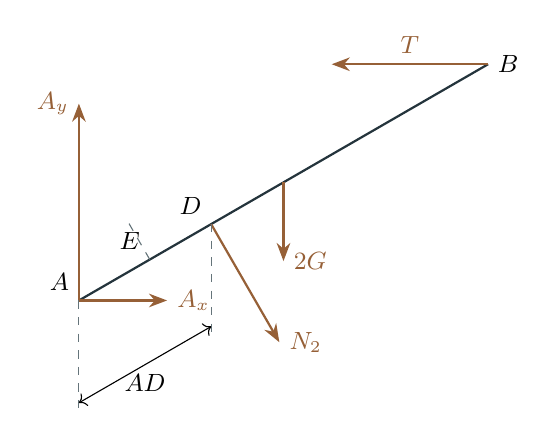
\begin{tikzpicture}
\coordinate(A)at(0,0);\coordinate(B)at(5.196152423,3);
\coordinate(E)at(.9,.519615242);\coordinate(F)at(1.939230485,1.119615242);
\coordinate(K)at(2.978460969,1.719615242);\coordinate(D)at(1.679422863,.969615242);
\draw[object](A)--(B);
\draw[force](B)--(3.210511777,3)node[midway,above]{$T$};
\draw[force](D)--(2.545448267,-.530384758)node[right]{$N_2$};
\draw[force](2.598076211,1.5)--(2.598076211,.5)node[right]{$2G$};
\draw[force](A)--(0,2.5)node[left]{$A_y$};
\draw[force](A)--(1.119615242,0)node[right]{$A_x$};
\draw[guide](E)--(.6,1.039230485);\node[above left]at(E){$E$};
\node[above left]at(D){$D$};\node[above left]at(A){$A$};\node[right]at(B){$B$};
\draw[guide](A)--(0,-1.4);\draw[guide](D)--(1.679422863,-.430384758);
\draw[<->](0,-1.3)--(1.679422863,-.330384758)node[midway,below]{$AD$};
\end{tikzpicture}
\figcaption{解图5.6B\quad 球对板的压力沿同一作用线反向；铰链两反力均保留，力矩臂按实际$L:R$绘制。}
\end{minipage}\end{center}
张力的力臂是 $L\sin30^\circ$，板重的力臂为 $(L/2)\cos30^\circ$，而球压力垂直板，力臂直接为 $AD$。故
\[
 TL\sin30^\circ=N_2AD+2G\frac L2\cos30^\circ.
\]
代入 $R/L=1/10$，逐项化简：
\begin{align*}
 \frac{TL}{2}
 &=2\sqrt3G\left(\sqrt3+\frac32\right)R
   +\frac{\sqrt3}{2}GL\\
 &=(6+3\sqrt3)GR+\frac{\sqrt3}{2}GL,\\
 T&=\left[2(6+3\sqrt3)\frac RL+\sqrt3\right]G
 =\boxed{\frac{6+8\sqrt3}{5}G}\approx3.97128G.
\end{align*}
\textbf{三个板支持力的合力位置。}从右球向左球依次列沿板方向平衡，球间压力依次为 $G/2,G$；三个球所受板支持力，从左到右为 $\sqrt3G,\sqrt3G/2,\sqrt3G/2$。它们作用于 $E,E+2R,E+4R$，加权平均位置为
\[
 AD=AE+\frac{(\sqrt3G/2)2R+(\sqrt3G/2)4R}{2\sqrt3G}
 =AE+\frac32R.
\]
\begin{center}\begin{minipage}{\linewidth}\centering
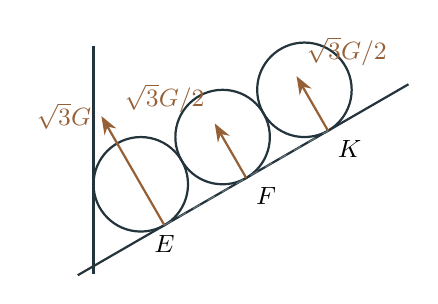
\begin{tikzpicture}
\coordinate(A)at(0,0);\coordinate(B)at(5.196152423,3);
\coordinate(E)at(.9,.519615242);\coordinate(F)at(1.939230485,1.119615242);
\coordinate(K)at(2.978460969,1.719615242);\coordinate(D)at(1.679422863,.969615242);
\draw[object](-.2,-.115470054)--(4,2.309401077);
\draw[object](0,-.1)--(0,2.8);
\foreach \x/\y in {.6/1.039230485,1.639230485/1.639230485,2.678460969/2.239230485}
{\draw[object](\x,\y)circle(.6);}
\draw[force](E)--(.1,1.905255888)node[left]{$\sqrt3G$};
\draw[force](F)--(1.539230485,1.812435565)node[above left]{$\sqrt3G/2$};
\draw[force](K)--(2.578460969,2.412435565)node[above right]{$\sqrt3G/2$};
\node[below]at(E){$E$};\node[below right]at(F){$F$};\node[below right]at(K){$K$};
\draw[guide](E)--(K);
\end{tikzpicture}
\figcaption{解图5.6C\quad 仅画待合成的三个法向力，作用点沿板相隔$2R$；逐球其他力由对应分量方程列出。}
\end{minipage}\end{center}
解图5.6C 把三个法向支持力按各自作用点合成，得到与整体取矩相同的作用点。木板的平移平衡给出铰链的竖直分力 $A_y=5G$ 和水平分力 $A_x=T-\sqrt3G$。
\subsubsection*{各球的法向力和切向平衡}
以$\vect t$沿板向右上、$\vect n$垂直板向左上，
三个球从左到右记为1、2、3，球间压力记为$P_{12},P_{23}$。
球间连心线与板平行，所以它们只在切向方程中出现。
先从最右球开始：
\[
P_{23}=G\sin30^\circ=\frac G2,\qquad
N_K=G\cos30^\circ=\frac{\sqrt3}2G.
\]
中球受到左球向右上的推力与右球向左下的推力，故
\[
P_{12}-P_{23}=G\sin30^\circ,\qquad
N_F=G\cos30^\circ,
\]
得到$P_{12}=G$、$N_F=\sqrt3G/2$。
左球另受水平墙力$N_1$，它的切向分量向板上，法向分量向板内：
\[
N_1\cos30^\circ-P_{12}-G\sin30^\circ=0,
\]
\[
N_E-N_1\sin30^\circ-G\cos30^\circ=0.
\]
逐式代入，恢复$N_1=\sqrt3G$、$N_E=\sqrt3G$。
所有球间压力与板支持力都为正，因此整体合成所使用的接触构型可以实现。
各球所受的接触法向力和重力都通过各自的圆心，对圆心的总力矩为零。

解图5.6C中，从左至右各垂足沿板的距离为
$AE,AE+2R,AE+4R$。三个法向力大小不同，合力位置用它们的大小作权重。三球质量相同，所以总重心位于中球的球心。
最右接触点距铰链为$(\sqrt3+4)R<10R=L$，
三个板接触点都在有限木板内，合力点$D$也在最左、最右接触点之间。

\subsubsection*{木板和三球整体的力矩}
这一选取会消去全部球板内力，外力中仍须保留墙对最左球的水平支持力。
令铰链$A$为坐标原点，三球中心的横坐标依次为
\[
R,\quad R+2R\cos30^\circ,\quad R+4R\cos30^\circ,
\]
墙力作用线的高度为$\sqrt3R$。
以逆时针为正，水平向右的墙力对$A$产生顺时针力矩，
球重和板重也产生顺时针力矩，只有$B$处向左的绳拉力产生逆时针力矩。
因此
\[
\begin{aligned}
TL\sin30^\circ
&=2G\frac L2\cos30^\circ+G(3R+6R\cos30^\circ)+N_1\sqrt3R\\
&=\frac{\sqrt3}{2}GL+(6+3\sqrt3)GR.
\end{aligned}
\]
与木板单独取矩中的$N_2AD$完全相同，故仍得$T=(6+8\sqrt3)G/5$。
墙力是板球整体的外力，它关于$A$的力矩为$3GR$，保留在整体矩方程中。

再回到三球重心$C$取矩：墙力作用线在$C$下方，水平向右，
所以它对$C$是逆时针；$D$在中球垂足$F$的左侧，
向左上的板合力对$C$是顺时针。
两力矩相抵才有$N_2FD=N_1R$。
同一墙力关于$A$和$C$的转向不同，因为两矩心分处其作用线两侧；
力矩方向由选定矩心与力的作用线共同决定。


\Needspace{18\baselineskip}

\pdfbookmark[2]{第 7 题 分段悬线的平衡与提升功}{q7}

\section*{第 7 题\quad 分段悬线的平衡与提升功}

\tagline{M-05-07}

四段质量可忽略的细线 $AB,BC,CD,DE$ 长度均为 $5\,\mathrm m$，$A,E$ 固定于同一水平天花板，$AE=14\,\mathrm m$。$B,D$ 各挂质量 $m_0=7\,\mathrm{kg}$ 的小球，$C$ 挂质量 $m$ 的重物。平衡构型关于 $C$ 的竖直线对称，$C$ 距天花板 $7\,\mathrm m$。
\begin{enumerate}\item 求 $m$。\item 用外力缓慢提升 $C$，直到 $B,C,D$ 在同一水平线上，求外力做的功。取 $g=9.8\,\mathrm{m/s^2}$。\end{enumerate}

\begin{center}\begin{minipage}{\linewidth}\centering
\begin{tikzpicture}
\draw[object] (-3.5,0)--(3.5,0);\draw[object] (-3.5,0)--(-2,-2)--(0,-3.5)--(2,-2)--(3.5,0);\foreach \x/\y/\s in {-3.5/0/A,3.5/0/E,-2/-2/B,2/-2/D,0/-3.5/C}{\fill(\x,\y)circle(2pt);\node[above right]at(\x,\y){$\s$};}\node[left]at(-2,-2.3){$m_0$};\node[right]at(2,-2.3){$m_0$};\node[below]at(0,-3.6){$m$};\draw[<->] (-3.5,.4)--(3.5,.4)node[midway,above]{$14\,\mathrm m$};\draw[<->] (4,0)--(4,-3.5)node[midway,right]{$7\,\mathrm m$};\node at(1.65,-3.1){各段 $5\,\mathrm m$};
\end{tikzpicture}
\figcaption{图 5.7\quad $A,E$ 固定在天花板，四段线均长 $5\,\mathrm m$，三个重物在节点 $B,C,D$。}
\end{minipage}\end{center}

\Needspace{5\baselineskip}\subsection*{解答}

\textbf{先由线长恢复节点位置。}以 $C$ 的竖直投影为水平原点，向右为正；以天花板为高度零，向上为正。于是 $A=(-7,0)$、$E=(7,0)$、$C=(0,-7)$。对称地设 $D=(u,-v)$，$B=(-u,-v)$。两段线长均为 $5\,\mathrm m$，给出
\[
 u^2+(7-v)^2=25,\qquad (7-u)^2+v^2=25.
\]
相减得 $u=v$。代回得
\[
 u^2+(7-u)^2=25,\qquad (u-3)(u-4)=0.
\]
几何有两支：$(u,v)=(3,3)$ 或 $(4,4)$。前一支的内段水平、竖直投影为 $3,4$，外段为 $4,3$，$D$ 点水平平衡给出 $T_2=3T_1/4$，竖直平衡却要求 $m_0g=3T_2/5-4T_1/5=-7T_1/20<0$，使节点所挂重量为负，因此取另一支。物理解为 $u=v=4$，所以 $B,D$ 离天花板 $4\,\mathrm m$。内段水平、竖直投影为 $4,3$，外段为 $3,4$。
\begin{center}\begin{minipage}{\linewidth}\centering
\begin{tikzpicture}
\draw[object] (-3.5,0)--(3.5,0);\draw[object] (-3.5,0)--(-2,-2)--(0,-3.5)--(2,-2)--(3.5,0);\foreach \x/\y/\s in {-3.5/0/A,3.5/0/E,-2/-2/B,2/-2/D,0/-3.5/C}{\fill(\x,\y)circle(2pt);\node[above right]at(\x,\y){$\s$};}\node[left]at(-2,-2.3){$m_0$};\node[right]at(2,-2.3){$m_0$};\node[below]at(0,-3.6){$m$};\draw[<->] (-3.5,.4)--(3.5,.4)node[midway,above]{$14\,\mathrm m$};\draw[<->] (4,0)--(4,-3.5)node[midway,right]{$7\,\mathrm m$};\node at(1.65,-3.1){各段 $5\,\mathrm m$};\draw[guide] (-3.5,0)--(-2.5,-2.291287847)--(2.5,-2.291287847)--(3.5,0);\node[below left]at(-2.5,-2.291287847){$B'$};\node[below right]at(2.5,-2.291287847){$D'$};\node[above]at(0,-2.291287847){$C'$};\draw[motion] (.15,-3.4)--(.15,-2.4);
\end{tikzpicture}
\figcaption{解图 5.7A\quad 实线为初态，虚线为终态；$C$ 上升，而 $B,D$ 下降。图上长度单位为 $2\,\mathrm m$。}
\end{minipage}\end{center}
\textbf{用两个节点确定质量。}解图5.7A区分初、末位置，计算提升功时各点高度须按各自位移取值。内段 $BC,CD$ 的张力为 $T_1$，外段 $AB,DE$ 为 $T_2$。解图5.7B中，$C$ 点竖直平衡、$D$ 点水平和竖直平衡分别为
\begin{align*}
 2T_1\frac35&=mg,\\
 T_1\frac45&=T_2\frac35,\\
 T_2\frac45-T_1\frac35&=m_0g.
\end{align*}
由第二式 $T_2=4T_1/3$，代入第三式：
\[
 \left(\frac{16}{15}-\frac35\right)T_1
 =\frac7{15}T_1=m_0g.
\]
故 $T_1=15m_0g/7$，$T_2=20m_0g/7$，再代入 $C$ 点方程：
\[
 m=\frac{2}{g}\frac35\frac{15m_0g}{7}
 =\frac{18}{7}m_0=\boxed{18\,\mathrm{kg}}.
\]
取 $g=9.8$，两种初态张力为 $147\,\mathrm N$ 和 $196\,\mathrm N$。
\begin{center}\begin{minipage}{\linewidth}\centering
\begin{tikzpicture}
\coordinate(C)at(0,0);\draw[force] (C)--(-1.2,.9)node[above left]{$T_1$};\draw[force] (C)--(1.2,.9)node[above right]{$T_1$};\draw[force] (C)--(0,-1.8)node[below]{$mg$};\node at(0,1.8){$C$ 节点};\begin{scope}[xshift=5cm]\draw[force] (0,0)--(-1.2,-.9)node[left]{$T_1$};\draw[force] (0,0)--(1.2,1.6)node[above]{$T_2$};\draw[force] (0,0)--(0,-.7)node[below]{$m_0g$};\node at(0,1.8){$D$ 节点};\end{scope}
\end{tikzpicture}
\figcaption{解图 5.7B\quad 初态内段的水平、竖直投影为 $4,3$；外段的投影为 $3,4$。}
\end{minipage}\end{center}
\textbf{终态三个节点一起移动。}当 $B',C',D'$ 水平时，内侧两段各长 $5\,\mathrm m$，所以 $B',D'$ 的横坐标为 $\mp5$。外侧线的水平投影为 $7-5=2$，故终态离天花板的深度为
\[
 v'=\sqrt{5^2-2^2}=\sqrt{21}\,\mathrm m.
\]
$C$ 上升 $7-\sqrt{21}$，$B,D$ 各下降 $\sqrt{21}-4$。中央重物的势能增加，两侧重物的势能减少。

\textbf{缓慢提升的外力功。}固定端不位移，约束力对整体无净功；缓慢过程的动能变化可忽略。因此外力功等于三个重物总重力势能的增加：
\begin{align*}
 W&=mg(7-\sqrt{21})+2m_0g(4-\sqrt{21})\\
 &=g\bigl[18(7-\sqrt{21})+14(4-\sqrt{21})\bigr]\\
 &=\boxed{g(182-32\sqrt{21})\,\mathrm{kg\,m}}
 \approx\boxed{346.504\,\mathrm J}.
\end{align*}
括号内的数值以 $\mathrm{kg\,m}$ 为单位。终态内段水平，张力的竖直分量为零，所以此时提升力为 $mg$。提升过程中内段方向持续变化，外力功等于各重物势能改变量之和。
\subsubsection*{提升途中是否仍能保持四段绷紧}
以天花板下方的中央深度为$H$，提升区间为
$\sqrt{21}\leq H\leq7$，所有长度以下按米取数值。
右节点为$D=(u,-v)$，仍有
\[
u^2+(H-v)^2=25,\qquad (7-u)^2+v^2=25.
\]
取与初态$(u,v)=(4,4)$连续的交点分支，令
\[
b(H)=\sqrt{\frac{51-H^2}{49+H^2}},
\qquad u=\frac{7+Hb}{2},\quad v=\frac{H+7b}{2}.
\]
代$H=7$给$u=v=4$，代$H=\sqrt{21}$给$u=5,v=\sqrt{21}$，
与解图5.7A初末构型一致。提升沿这一连续分支进行，另一交点在初态要求负张力。
对右节点重新列水平、竖直分量：
\[
T_1u=T_2(7-u),\qquad
T_2v-T_1(H-v)=5m_0g.
\]
因此
\[
T_1=\frac{5m_0g(7-u)}{7v-H(7-u)},\qquad
T_2=\frac{5m_0g\,u}{7v-H(7-u)}.
\]
这段提升中$4\leq u\leq5<7$，共同分母为
$(49+H^2)b/2>0$，所以两种张力始终为正，四段线都可保持绷紧。
在终态，内线虽水平，仍有
\[
T_{1f}=\frac{2m_0g}{\sqrt{21}},\qquad
T_{2f}=\frac{5m_0g}{\sqrt{21}}.
\]
终态的内线仍有张力，方向沿水平，其竖直分量为零。

\subsubsection*{变力做功与势能法的对应}
提升量为$s=7-H$。由势能函数的导数求准静态外力，
\[
F_\uparrow=\frac{\dd W}{\dd s}
=mg+2m_0g\,\frac{\dd v}{\dd H},
\]
\[
\frac{\dd v}{\dd H}
=\frac12-\frac{350H}{(49+H^2)^{3/2}\sqrt{51-H^2}}.
\]
在初态该导数为$-9/7$，因$m/m_0=18/7$，$F_\uparrow=0$；
在终态导数为零，$F_\uparrow=mg$。
两者之间外力逐渐增大，解图5.7C给出完整曲线。
\begin{center}\begin{minipage}{\linewidth}\centering
\begin{tikzpicture}[x=2cm,y=1cm]
\draw[axis](0,0)--(2.85,0)node[right]{$s/\mathrm m$};
\draw[axis](0,0)--(0,3.3)node[above]{$F_\uparrow/(m_0g)$};
\draw[traj,domain=0:2.417424305,samples=120]
plot(\x,{25/7-700*(7-\x)/((49+(7-\x)^2)^1.5*sqrt(51-(7-\x)^2))});
\draw[guide](0,18/7)--(2.417424305,18/7)--(2.417424305,0);
\node[left]at(0,18/7){$18/7$};\node[below]at(2.417424305,0){$7-\sqrt{21}$};
\node[above left]at(2.417424305,18/7){$F_\uparrow=mg$};
\end{tikzpicture}
\figcaption{解图5.7C\quad 准静态提升力从零增到$mg$；以 $s/\mathrm m$ 为横坐标时，曲线下面积乘 $m_0g\cdot 1\,\mathrm m$ 给出外力功。}
\end{minipage}\end{center}
直接积分也有
\[
\begin{aligned}
\int_0^{7-\sqrt{21}}F_\uparrow\,\dd s
&=\int_{\sqrt{21}}^7
\left(mg+2m_0g\frac{\dd v}{\dd H}\right)\dd H\\
&=mg(7-\sqrt{21})+2m_0g(4-\sqrt{21}).
\end{aligned}
\]
恢复与势能法相同的功，侧球下降贡献的负项没有消失。
理想轻绳每段的两端速度在绳方向上的投影相同，
该段张力在两个节点处所做的功相消；固定端又无位移，
所以把三个质量一起计算时无需再加绳张力的功。



\Needspace{18\baselineskip}

\pdfbookmark[2]{第 8 题 浮子与插杆的稳定性}{q8}

\section*{第 8 题\quad 浮子与插杆的稳定性}

\tagline{M-05-08}

浮子由两个相同的均匀球冠合成，两个球冠密度相同、曲率半径均为 $R$。浮子质量为 $m_1$，中心厚度为 $h<2R$。一根长为 $l$、质量为 $m_2$ 的均匀细杆沿浮子轴线插入，下端恰到下球冠的最低点。杆竖直时系统平衡。按图中的浸没构型，浸水表面在下球冠内，小偏转时液面不越过两球冠接缝。分析竖直平衡的稳定性。

\begin{center}\begin{minipage}{\linewidth}\centering
\begin{tikzpicture}
\draw[object](-1.428285686,.6)arc(224.427004001:315.572995999:2);
\draw[object](-1.428285686,.6)arc(135.572995999:44.427004001:2);
\draw[object,line width=1.3pt](0,0)--(0,4.5);
\draw[accent](-2.2,.2)--(2,.2)node[right]{液面};
\fill(0,0)circle(1.7pt)node[below]{$S$};
\fill(0,2)circle(1.7pt)node[left]{$O$};
\draw[<->](.65,0)--(.65,2)node[midway,right]{$R$};
\node[left]at(0,3.5){$l,m_2$};\node[left]at(-1.2,.6){$m_1$};
\draw[<->](-1.9,0)--(-1.9,1.2)node[midway,left]{$h$};
\end{tikzpicture}
\figcaption{图5.8\quad $SO=R$为下球冠曲率半径，浮子中心厚度为$h$；液面处于下球冠内。}
\end{minipage}\end{center}

\Needspace{5\baselineskip}\subsection*{解答}

\textbf{先确定浮力作用线。}设下球冠最低点为 $S$，其曲率中心为 $O$，$SO=R$。浮子重心 $C_1$ 距 $S$ 为 $h/2$，均匀杆重心 $C_2$ 距 $S$ 为 $l/2$，三个点都在系统轴线上。

在题给浸没范围内，浸水表面属于同一球面。每个液体压力沿球面法线，作用线都经过 $O$，故浮力合力的作用线也经过 $O$。静止时浮力大小为 $(m_1+m_2)g$；判断小偏转时的力矩，只需比较组合重心 $C$ 与 $O$ 的位置。
\begin{center}\begin{minipage}{\linewidth}\centering
\begin{tikzpicture}
\coordinate(O)at(0,1.9);\draw[guide] (0,-.4)--(0,4);\begin{scope}[shift={(0,1.9)},rotate=-13]\coordinate(S)at(0,-2);\coordinate(C)at(0,-.6);\draw[object] (-1.428285686,-1.4)arc(224.427004001:315.572995999:2);\draw[object] (-1.428285686,-1.4)arc(135.572995999:44.427004001:2);\draw[object,line width=1.3pt] (0,-2)--(0,2.5);\draw[<->] (.5,-.6)--(.5,0)node[midway,right]{$x$};\end{scope}\fill(O)circle(2pt);\fill(C)circle(2pt);\node[left]at(O){$O$};\node[left]at(C){$C$};\node[below]at(S){$S$};\draw[force] (O)--(0,3.2)node[right]{$F_b$};\draw[force] (C)--++(0,-1)node[right]{$(m_1+m_2)g$};\draw (0,2.6)arc(90:77:.7);\node at(.26,2.85){$\alpha$};\draw[accent] (-2.2,.1)--(1.8,.1)node[right]{液面};\node[align=left]at(3.8,1.7){图示 $x>0$\\重心低于曲率中心\\小偏转产生恢复力矩};
\end{tikzpicture}
\figcaption{解图 5.8A\quad $O$ 是下球冠的曲率中心，$C$ 是组合重心；浮力作用线经过 $O$，$x=R-SC$。}
\end{minipage}\end{center}
解图5.8A中，先沿倾斜轴由最低点$S$量出组合重心$C$，再与曲率中心$O$比较。浮力经过$O$，对$O$取矩只需保留作用在$C$的重力；图中$x=R-SC$是有符号距离，$x>0$表示$C$在$O$下方。解图5.8B中同向偏转的三个构型，正好对应恢复、失稳和中性三种力矩。

\textbf{组合重心。}以 $S$ 为轴向坐标零点，向杆上端为正，得到
\[
 SC=\frac{m_1(h/2)+m_2(l/2)}{m_1+m_2}
 =\frac{m_1h+m_2l}{2(m_1+m_2)}.
\]
定义有符号距离
\[
 x=R-SC
 =R-\frac{m_1h+m_2l}{2(m_1+m_2)}.
\]
$x>0$ 表示重心低于曲率中心，$x<0$ 表示高于曲率中心。

\textbf{偏转时浮子与杆的重力矩。}让轴线顺时针偏离竖直一个小角 $\alpha>0$，取增加 $\alpha$ 的转向为正。浮力对 $O$ 的力矩为零。先分别写浮子和杆的重力矩，保留力臂的符号：
\[
 \tau_1=-m_1g\left(R-\frac h2\right)\sin\alpha,
 \qquad
 \tau_2=-m_2g\left(R-\frac l2\right)\sin\alpha.
\]
若 $l/2>R$，杆的力矩使偏角增大；若 $l/2<R$，杆也有恢复作用。两者相加，得到组合重力的力矩
\[
 \tau=-(m_1+m_2)g\,x\sin\alpha
 \simeq-(m_1+m_2)g\,x\alpha.
\]
当 $x>0$，重力使 $\alpha$ 减小，是恢复力矩；当 $x<0$，重力使偏角增大，是偏离力矩。于是
\[
 \boxed{\begin{aligned}
 m_1h+m_2l&<2R(m_1+m_2)&&\text{稳定},\\
 m_1h+m_2l&>2R(m_1+m_2)&&\text{不稳定},\\
 m_1h+m_2l&=2R(m_1+m_2)&&\text{随遇平衡}.
 \end{aligned}}
\]
\begin{center}\begin{minipage}{\linewidth}\centering
\begin{tikzpicture}
\foreach \j/\yy/\ss in {0/-.8/{稳定},1/0/{随遇},2/.8/{不稳定}}{\begin{scope}[xshift={4*\j cm}]\draw[guide] (0,-1.3)--(0,1.6);\draw[object] (-.28,-1.2)--(.28,1.2);\fill(0,0)circle(2pt);\coordinate(C)at({.233*\yy},\yy);\fill(C)circle(2pt);\draw[force] (C)--++(0,-.7);\ifnum\j=1\node[left]at(0,0){$O=C$};\else\node[left]at(0,0){$O$};\node[right]at(C){$C$};\fi\node at(0,2){\ss};\end{scope}}\node at(0,-1.9){$x>0,\ \tau\alpha<0$};\node at(4,-1.9){$x=0,\ \tau=0$};\node at(8,-1.9){$x<0,\ \tau\alpha>0$};
\end{tikzpicture}
\figcaption{解图 5.8B\quad 统一取顺时针偏角为正，组合重心的位置决定小偏转后力矩的符号。}
\end{minipage}\end{center}
等号时 $C=O$。在这一浸没构型内，重力和浮力在有限小偏转时仍沿同一条竖直线，对 $O$ 的力矩恒为零，因而是随遇平衡。

\textbf{偏转势能与临界杆长。}球面浸水体积不变时，$O$ 的平衡高度不随小偏角改变。有效势能的变化可写为
\[
 U(\alpha)-U(0)=(m_1+m_2)gx(1-\cos\alpha),
\]
其极小、极大或常值与上面的力矩结论相同。临界杆长为
\[
 \boxed{l_c=2R+\frac{m_1}{m_2}(2R-h)}.
\]
因 $h<2R$，临界杆长 $l_c>2R$。若 $l\le2R$，浮子的重心低于 $O$，杆的重心在 $O$ 或更低，组合重心在 $O$ 下方，因而稳定。这个判据对应液面始终截在球冠内的情形。若液面越过接缝，浮力作用线由新浸没形状的浮心或稳心确定。
\subsubsection*{把两个重心与各自力矩画在同一图中}
解图5.8C另画浮子重心$C_1$和杆重心$C_2$。
在这个示例中，$C_1$位于$O$下方，$C_2$略高于$O$；
两支重力都向下，各自的作用线分处 $O$ 的左右两侧，因此力矩转向相反。
\begin{center}\begin{minipage}{\linewidth}\centering
\begin{tikzpicture}
\coordinate(O)at(0,0);\draw[guide](0,-2.25)--(0,2.8);
\begin{scope}[rotate=-13]
\coordinate(S)at(0,-2);\coordinate(Cone)at(0,-1.4);
\coordinate(Ctwo)at(0,.25);\coordinate(C)at(0,-.6);
\draw[object](-1.428285686,-1.4)arc(224.427004001:315.572995999:2);
\draw[object](-1.428285686,-1.4)arc(135.572995999:44.427004001:2);
\draw[object,line width=1.3pt](0,-2)--(0,2.5);
\end{scope}
\foreach \p/\lab in {O/O,S/S,Cone/C_1,C/C}
{\fill(\p)circle(1.6pt);\node[left]at(\p){$\lab$};}
\fill(Ctwo)circle(1.6pt);\draw[guide](Ctwo)--(.6,.55);
\node[right]at(.6,.55){$C_2$};
\draw[force](Cone)--++(0,-.68)node[right]{$m_1g$};
\draw[force](Ctwo)--++(0,-.64)node[right]{$m_2g$};
\draw[accent](-2.1,-1.8)--(1.8,-1.8)node[right]{液面};
\draw[force](O)--(0,1.3)node[left]{$F_b$};
\node[align=left,anchor=west]at(2.3,.6){$C_1$的重力恢复\\$C_2$的重力倾覆\\比较质量与力臂的乘积};
\end{tikzpicture}
\figcaption{解图5.8C\quad 示例$R=2,h=1.2,l=4.5,m_1:m_2=17:16$；合重心仍低于$O$，两个重力矩按质量乘各自力臂计算。}
\end{minipage}\end{center}
该示例从$S$算出的两重心高度为$h/2=0.6$、$l/2=2.25$，
所以$SC=(17\times0.6+16\times2.25)/33=1.4<R=2$。
尽管杆重心已超过曲率中心，组合体仍有$x=0.6>0$的恢复力臂。
在这个构型中，浮子重力的恢复力矩大于杆重力的倾覆力矩，两力矩相加仍指向竖直位置。

\subsubsection*{排水体积与球冠浸没范围}
稳定判据建立在题给浸没构型已存在的前提下。
若另给液体密度$\rho_\ell$，令竖直状态液面距下球面最低点的高度为$d$，
在下球冠内须$0<d<h/2$。
球缺排水体积与漂浮条件为
\[
V(d)=\pi d^2\left(R-\frac d3\right),\qquad
m_1+m_2=\rho_\ell V(d).
\]
因此要使液面严格低于接缝，应有
\[
0<m_1+m_2<
\rho_\ell\pi\left(\frac h2\right)^2
\left(R-\frac h6\right).
\]
若总质量超过这个范围，物体仍可能在更深浸没下漂浮，
但浸水表面不再全属于下球冠，就需要另一套浮力线分析。
当液面仍截在下球冠内时，组合重心相对 $O$ 的位置决定恢复力矩。

小倾角后，排水体积仍由同一球面截出的球缺给出，
保持排水体积使$d$不变，也使$O$到水平液面的距离不变。
因此在势能式中，$O$ 的平衡高度与小偏角无关。
令$c=R-h/2$、接缝圆半径$a=\sqrt{R^2-c^2}$，
倾斜$\alpha$后接缝最低点相对$O$的竖直坐标为
$-c\cos\alpha-a|\sin\alpha|$。
在足够小的偏角内，液面不跨缝可由
\[
d<R-c\cos\alpha-a|\sin\alpha|
\]
保证。$\alpha=0$时恢复$d<h/2$；
只要初态保留严格余量，就存在一段非零的小偏转范围可沿用球面模型。
等号稳定情形中所说的随遇，也限于这个构型保持不变的范围。


\Needspace{18\baselineskip}

\pdfbookmark[2]{第 9 题 五杆悬挂的平衡形状}{q9}

\section*{第 9 题\quad 五杆悬挂的平衡形状}

\tagline{M-05-09}

五根质量均匀、质量和长度完全相同的细杆，用光滑铰链首尾相连成五边形，从一个顶点悬挂。求图示对称平衡构型的五个内角。铰链只传递力，不传递力矩。

\begin{center}\begin{minipage}{\linewidth}\centering
\begin{tikzpicture}
\coordinate(O)at(0,0);
\coordinate(A)at(.514173628485,-2.955609155448);
\coordinate(B)at(1.5,-5.789007532879);
\coordinate(C)at(-1.5,-5.789007532879);
\coordinate(D)at(-.514173628485,-2.955609155448);
\draw[object](O)--(A)--(B)--(C)--(D)--cycle;
\draw[guide](0,.25)--(0,-6.1);
\foreach \p/\pos in {O/above,A/right,B/below right,C/below left,D/left}
{\fill(\p)circle(1.6pt);\node[\pos]at(\p){$\p$};}
\node[right]at(2.4,-3.4){各杆$l,m$相同};
\end{tikzpicture}
\figcaption{图5.9\quad 悬点$O$固定，五根等长等重杆按左右对称构型闭合。}\end{minipage}\end{center}

\Needspace{5\baselineskip}\subsection*{解答}

\textbf{变量与闭合条件。}设每杆长 $l$、质量 $m$。顶悬点为 $O$，右侧两杆依次为 $OA,AB$，底杆为 $BC$。令上、下侧杆与向下竖直线的夹角为 $\varphi_1,\varphi_2$，两杆都向右下方延伸。底杆水平，右半宽等于 $l/2$，所以
\[
 l\sin\varphi_1+l\sin\varphi_2=\frac l2,
 \qquad \sin\varphi_1+\sin\varphi_2=\frac12.\tag{1}
\]
\begin{center}\begin{minipage}{\linewidth}\centering
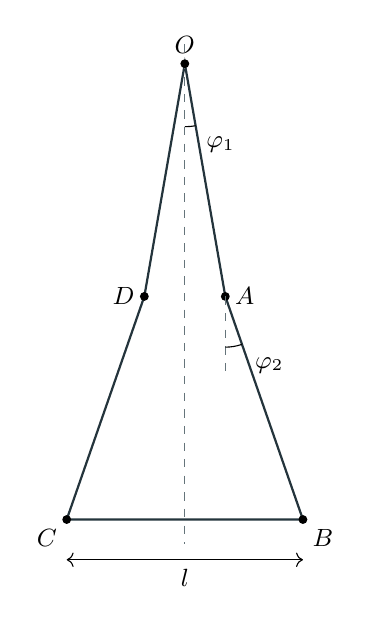
\begin{tikzpicture}
\coordinate(O)at(0,0);
\coordinate(A)at(.514173628485,-2.955609155448);
\coordinate(B)at(1.5,-5.789007532879);
\coordinate(C)at(-1.5,-5.789007532879);
\coordinate(D)at(-.514173628485,-2.955609155448);
\draw[object](O)--(A)--(B)--(C)--(D)--cycle;
\draw[guide](0,.25)--(0,-6.1);
\foreach \p/\pos in {O/above,A/right,B/below right,C/below left,D/left}
{\fill(\p)circle(1.6pt);\node[\pos]at(\p){$\p$};}
\draw[guide](A)--(.514173628485,-4);
\draw(0,-.8)arc(-90:-80.131283233:.8);\node[right]at(.15,-1.03){$\varphi_1$};
\draw(.514173628485,-3.6)arc(-90:-70.815643521:.644390845);
\node[right]at(.77,-3.83){$\varphi_2$};
\draw[<->](-1.5,-6.3)--(1.5,-6.3)node[midway,below]{$l$};
\end{tikzpicture}
\figcaption{解图5.9A\quad 依未平方方程的数值解绘制，每边等长；两侧顶点是凹角。}\end{minipage}\end{center}
\textbf{逐杆取矩。}按解图5.9A的凹形构型从底杆往上分析。底杆两端各受向上的 $mg/2$；它的水平端力大小记为 $T$。各杆没有其他水平外力，因此这个水平分力沿右半链保持不变。竖直分力由下向上逐杆增加：下侧杆下端为 $mg/2$、上端为 $3mg/2$；上侧杆下端为 $3mg/2$、上端为 $5mg/2$。解图5.9B画的是每根杆所受的端力，相邻两杆在共同铰链处的作用力反向。
\begin{center}\begin{minipage}{\linewidth}\centering
\begin{tikzpicture}
\coordinate(A)at(.514173628485,-2.955609155448);
\draw[object](0,0)--(A);
\draw[force](0,0)--(-.208758439,0)node[left]{$T$};
\draw[force](0,0)--(0,1.5)node[right]{$5mg/2$};
\draw[force](A)--(.722932068,-2.955609155448)node[right]{$T$};
\draw[force](A)--(.514173628485,-3.855609155448)node[right]{$3mg/2$};
\draw[force](.257086814242,-1.477804577724)--(.257086814242,-2.077804577724)node[left]{$mg$};
\node at(1.6,-1){上侧杆};
\begin{scope}[xshift=4.5cm]
\coordinate(B)at(.985826371515,-2.833398377431);
\draw[object](0,0)--(B);
\draw[force](0,0)--(-.208758439,0)node[left]{$T$};
\draw[force](0,0)--(0,.9)node[right]{$3mg/2$};
\draw[force](B)--(1.194584811,-2.833398377431)node[right]{$T$};
\draw[force](B)--(.985826371515,-3.133398377431)node[right]{$mg/2$};
\draw[force](.492913185758,-1.416699188716)--(.492913185758,-2.016699188716)node[left]{$mg$};
\node at(2,-1){下侧杆};
\end{scope}
\end{tikzpicture}
\figcaption{解图5.9B\quad 杆方向及各端力依平衡解绘制；同一铰链在相邻两杆上按作用反作用反向。}
\end{minipage}\end{center}
对上侧杆的上端 $O$ 取矩，得
\[
 Tl\cos\varphi_1
 =\frac32mg\,l\sin\varphi_1
  +mg\frac l2\sin\varphi_1,
 \quad T=2mg\tan\varphi_1.
\]
对下侧杆的上端 $A$ 取矩，得
\[
 Tl\cos\varphi_2
 =\frac12mg\,l\sin\varphi_2
  +mg\frac l2\sin\varphi_2,
 \quad T=mg\tan\varphi_2.
\]
消去 $T$：
\[
 \tan\varphi_2=2\tan\varphi_1.\tag{2}
\]
\textbf{数值求解与物理解。}令 $x=\sin\varphi_1$。由(2)，在 $0<\varphi_i<\pi/2$ 内
\[
 \sin\varphi_2=\frac{2x}{\sqrt{1+3x^2}}.
\]
代入(1)，得
\[
 q(x):=x+\frac{2x}{\sqrt{1+3x^2}}-\frac12=0,
 \qquad 0<x<\frac12.
\]
因 $q'(x)=1+2/(1+3x^2)^{3/2}>0$，且 $q(0)<0,q(1/2)>0$，物理解唯一。平方展开也可得到
\[
 12x^4-12x^3-9x^2-4x+1=0,
\]
但须代回未平方的方程筛根。采用二分或牛顿迭代
\[
 x_{k+1}=x_k-
 \frac{x_k+2x_k/\sqrt{1+3x_k^2}-1/2}
 {1+2/(1+3x_k^2)^{3/2}},
\]
从 $x_0=0.17$ 出发，迭代值依次为
\[
 x_0=0.17000000,\qquad x_1=0.17139034,\qquad x_2=0.17139121.
\]
代回未平方方程得到 $q(x_2)$ 接近零，进而
\[
 \varphi_1\simeq9.869^\circ,\qquad
 \varphi_2\simeq19.184^\circ.
\]
五个内角依次为
\[
 \boxed{\begin{aligned}
 \angle O&=2\varphi_1\simeq19.737^\circ,\\
 \angle A=\angle D&=180^\circ+\varphi_2-\varphi_1
 \simeq189.316^\circ,\\
 \angle B=\angle C&=90^\circ-\varphi_2\simeq70.816^\circ.
 \end{aligned}}
\]
侧角大于 $180^\circ$，表示凹顶点；取五边形内部的凹角，五角和仍为$540^\circ$。

\Needspace{12\baselineskip}\textbf{另解：按闭合约束求势能极小。}以 $O$ 为高度零点。两根上侧杆重心深度各为 $l\cos\varphi_1/2$；两根下侧杆各为 $l\cos\varphi_1+l\cos\varphi_2/2$；底杆重心深度为 $l(\cos\varphi_1+\cos\varphi_2)$。相加得
\[
 U=-2mgl(2\cos\varphi_1+\cos\varphi_2).
\]
由(1)微分：$\dd\varphi_2/\dd\varphi_1=-\cos\varphi_1/\cos\varphi_2$，故
\[
 \frac{\dd U}{\dd\varphi_1}
 =2mgl\cos\varphi_1(2\tan\varphi_1-\tan\varphi_2).
\]
令其为零仍得(2)。在约束下增大 $\varphi_1$ 会减小 $\varphi_2$，括号内表达式严格增大，所以导数由负转正，这个构型在所用的对称变形路径上是势能极小。
\subsubsection*{四次方程的逐步消元}
若用多项式求根，须把平方前后的条件都保留。
由$\tan\varphi_2=2\tan\varphi_1$，平方后有
\[
\frac{\sin^2\varphi_2}{1-\sin^2\varphi_2}
=\frac{4x^2}{1-x^2},
\quad
\sin^2\varphi_2(1+3x^2)=4x^2.
\]
宽度闭合又给$\sin\varphi_2=1/2-x$，所以
\[
\left(\frac12-x\right)^2(1+3x^2)=4x^2,
\]
\[
(1-4x+4x^2)(1+3x^2)=16x^2.
\]
展开左端并移项，才得到
\[
f(x)=12x^4-12x^3-9x^2-4x+1=0.
\]
$0<x<1/2$同时保证两个倾角都在第一象限、$1/2-x>0$，
因而这个区间内平方不会改变所取正根的符号。
从四次式求得候选根后，取 $0<x<1/2$ 内同时满足未平方方程 $q(x)=0$ 和闭合式的根，由此恢复 $\varphi_1,\varphi_2$。两杆的方向和宽度闭合共同确定这个区间，它比 $0\leq\sin\varphi_1\leq1$ 更窄。

二分定位用到的多项式值为
\[
\begin{array}{c|r|r}
x&f(x)&q(x)\\ \hline
0.10&0.499200&-0.202934\\
0.15&0.163075&-0.059640\\
0.17&0.010967&-0.003845\\
0.17139000&0.000009556&-0.000003341\\
0.17139121&-0.000000004&0.0000000014\\
0.20&-0.236800&0.077964
\end{array}
\]
二分先把根夹在$0.1$与$0.2$之间，再缩到$0.17139$附近；
牛顿法利用同一初始区间加快收敛，两种算法趋向同一个物理解。
因为$q'(x)>1$，在包含根的区间内由中值定理有
$|x-x_*|\leq|q(x)|$，可用未平方残差直接控制根的误差。
保留足够位数以后再换算角度，避免先把$x$取到四位就报告毫度精度。

\subsubsection*{把数值形状代回逐杆受力}
求根得$x_*=0.17139120949494\ldots$，
$\sin\varphi_2=0.32860879050506\ldots$。两条力矩式分别给
\[
\frac{T}{mg}=2\tan\varphi_1
=\tan\varphi_2=0.3479307320\ldots.
\]
两式求得的是同一水平铰链分力，两根杆端的竖直分力各自由受力方程确定。
下侧杆上端竖直分力$3mg/2$、下端$mg/2$相差恰为自身重量，
上侧杆的$5mg/2$、$3mg/2$也相差$mg$。
底杆两端向上的$mg/2$恰好承担本杆重量，
两侧向内的水平力使底杆受压，刚杆通过两端的铰链传递这一压力。

解图5.9B按这组解画出杆方向与铰链作用点。
在右上杆上，下端力为$(T,-3mg/2)$；
在右下杆上，同一铰链处的力为$(-T,3mg/2)$。
两个力作用于不同杆，合并成整体时才相消。
悬点的两份向上分力各$5mg/2$相加为$5mg$，
左右水平分力相消，符合全系统悬挂平衡。
因此各杆的局部平衡、底杆承压和整体承重均由同一组力满足。

按每杆长$l$重画时，
$OA=AB=BC=CD=DO=l$，横向闭合仍是$OB_x=l/2$。
侧顶点比从$O$到$B$的直线更靠近对称轴，所以这里确是凹五边形。
五角之和的精确关系为
\[
2\varphi_1+
2(180^\circ+\varphi_2-\varphi_1)+
2(90^\circ-\varphi_2)=540^\circ.
\]


\subsubsection*{对称变形下的势能曲率}
在驻点处，$2\tan\varphi_1-\tan\varphi_2=0$，
故前面势能一阶导数再微分时，乘$\sin\varphi_1$的一项消失，得到
\[
\left.\frac{\dd^2U}{\dd\varphi_1^2}\right|_{\rm eq}
=2mgl\cos\varphi_1
\left(\frac{2}{\cos^2\varphi_1}
+\frac{\cos\varphi_1}{\cos^3\varphi_2}\right)>0.
\]
正的二阶导数表明，在对称闭合路径上该驻点是势能极小。
每杆都具有同一$m,l$，两者只成为势能的公共比例和铰链力的量纲因子，
所以共同放大质量或长度不会改变求出的五角。
若只改变某杆质量，竖直分力分配改变，便不能继续保留同一角度。
这里的二阶计算仍只涉及所选对称路径；若要讨论任意非对称扰动，须另保留那些独立自由度。


\Needspace{18\baselineskip}

\pdfbookmark[2]{第 10 题 厚木板在圆柱上的稳定性}{q10}

\section*{第 10 题\quad 厚木板在圆柱上的稳定性}

\tagline{M-05-10}

半径为 $R$ 的圆柱固定在水平地面上。厚度为 $t$ 的均匀木板水平放置在圆柱顶部，木板长度方向垂直于圆柱轴线，木板中线位于圆柱正上方。接触处有静摩擦，使微小偏转中木板与圆柱不滑动。求水平平衡稳定的厚度条件，并判别临界厚度。

\begin{center}\begin{minipage}{\linewidth}\centering
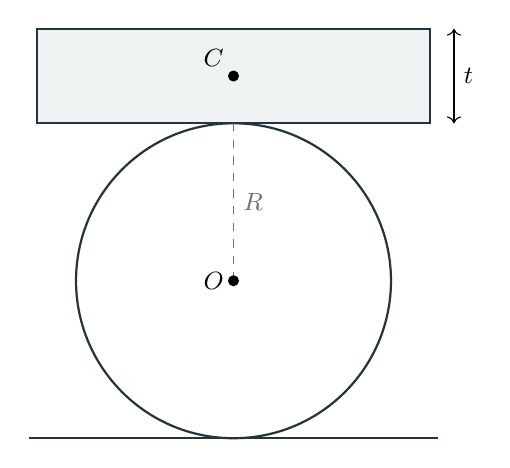
\begin{tikzpicture}
\draw[object](0,0)circle(2);\draw[object,fill=rulegray!35](-2.5,2)rectangle(2.5,3.2);
\draw[object](-2.6,-2)--(2.6,-2);
\draw[guide](0,0)--(0,2)node[midway,right]{$R$};
\draw[<->](2.8,2)--(2.8,3.2)node[midway,right]{$t$};
\fill(0,0)circle(2pt)node[left]{$O$};
\fill(0,2.6)circle(2pt)node[above left]{$C$};
\end{tikzpicture}
\figcaption{图5.10\quad 均匀板水平放在圆柱上，$C$在板截面中点，微小偏转遵守无滑动约束。}
\end{minipage}\end{center}

\Needspace{5\baselineskip}\subsection*{解答}

\textbf{随偏转移动的接触点。}设圆柱中心为 $O$，木板中线与下表面的交点为材料点 $P$，木板重心为 $C$，$PC=t/2$。水平时 $P$ 正好是接触点。木板向右偏转 $\theta$ 后，新接触点为 $M$，半径 $OM$ 也偏离竖直 $\theta$。

无滑动约束使圆柱上经过的弧长等于板下表面经过的长度，所以
\[
 MP=R\theta.
\]
解图5.10A中，从 $O$ 到 $M$ 的竖直投影为 $R\cos\theta$；沿板由 $M$ 到 $P$ 的投影为 $R\theta\sin\theta$；由 $P$ 到 $C$ 的投影为 $(t/2)\cos\theta$。重心高度因此为
\[
 z_C(\theta)=\left(R+\frac t2\right)\cos\theta
              +R\theta\sin\theta.
\]
\begin{center}\begin{minipage}{\linewidth}\centering
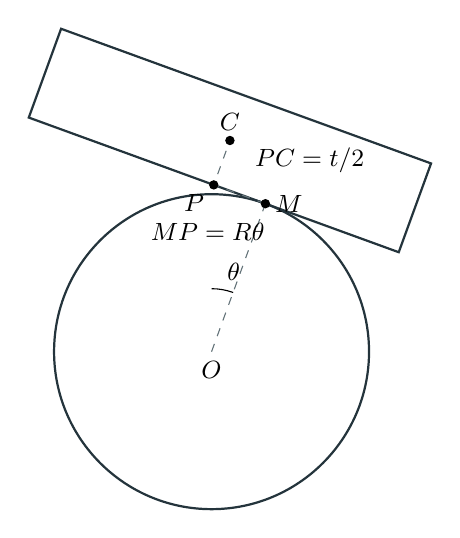
\begin{tikzpicture}
\pgfmathsetmacro{\th}{20}\pgfmathsetmacro{\radth}{rad(\th)}
\coordinate(O)at(0,0);\coordinate(M)at({2*sin(\th)},{2*cos(\th)});
\coordinate(P)at({2*sin(\th)-2*\radth*cos(\th)},{2*cos(\th)+2*\radth*sin(\th)});
\coordinate(C)at({2.6*sin(\th)-2*\radth*cos(\th)},{2.6*cos(\th)+2*\radth*sin(\th)});
\draw[object](O)circle(2);
\draw[object]
({2*sin(\th)-(2*\radth+2.5)*cos(\th)},{2*cos(\th)+(2*\radth+2.5)*sin(\th)})
--({2*sin(\th)-(2*\radth-2.5)*cos(\th)},{2*cos(\th)+(2*\radth-2.5)*sin(\th)})
--({3.2*sin(\th)-(2*\radth-2.5)*cos(\th)},{3.2*cos(\th)+(2*\radth-2.5)*sin(\th)})
--({3.2*sin(\th)-(2*\radth+2.5)*cos(\th)},{3.2*cos(\th)+(2*\radth+2.5)*sin(\th)})--cycle;
\draw[guide](O)--(M);\draw[guide](M)--(P)--(C);
\foreach \p in {M,P,C}{\fill(\p)circle(1.7pt);}
\node[right]at(M){$M$};\node[below left]at(P){$P$};\node[above]at(C){$C$};
\node[below]at(O){$O$};\node[below]at(-.05,1.75){$MP=R\theta$};
\node[right]at(.43,2.43){$PC=t/2$};
\draw(0,.8)arc(90:70:.8);\node at(.28,1.02){$\theta$};
\end{tikzpicture}
\figcaption{解图5.10A\quad 按无滑动坐标画出整块板，材料点$P$在下表面中点，$C$在实际截面中心。}
\end{minipage}\end{center}
\textbf{势能的二阶项和四阶项。}木板质量记为 $m$。势能 $U=mgz_C$，而
\begin{align*}
 \cos\theta&=1-\frac{\theta^2}{2}+\frac{\theta^4}{24}
              +O(\theta^6),\\
 \theta\sin\theta&=\theta^2-\frac{\theta^4}{6}
              +O(\theta^6).
\end{align*}
代入得
\[
 U(\theta)-U(0)
 =mg\left[\frac12\left(R-\frac t2\right)\theta^2
       +\left(\frac t{48}-\frac R8\right)\theta^4
       +O(\theta^6)\right].
\]
若 $t<2R$，最低非零项为正的二阶项，重心在偏转后升高，水平状态为势能极小，稳定。若 $t>2R$，二阶项为负，偏转降低重心，不稳定。
\begin{center}\begin{minipage}{\linewidth}\centering
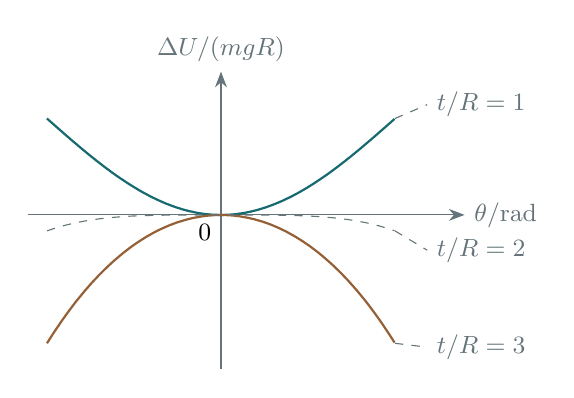
\begin{tikzpicture}[x=3.4cm,y=14cm]
\draw[axis](-.72,0)--(.91,0)node[right]{$\theta/\mathrm{rad}$};
\draw[axis](0,-.14)--(0,.13)node[above]{$\Delta U/(mgR)$};
\draw[traj,domain=-.65:.65,samples=120]plot(\x,{1.5*(cos(deg(\x))-1)+\x*sin(deg(\x))});
\draw[object,color=warm,domain=-.65:.65,samples=120]plot(\x,{2.5*(cos(deg(\x))-1)+\x*sin(deg(\x))});
\draw[muted,dashed,domain=-.65:.65,samples=120]plot(\x,{2*(cos(deg(\x))-1)+\x*sin(deg(\x))});
\draw[guide](.65,{1.5*(cos(deg(.65))-1)+.65*sin(deg(.65))})--(.77,.10)node[right]{$t/R=1$};
\draw[guide](.65,{2*(cos(deg(.65))-1)+.65*sin(deg(.65))})--(.77,-.032)node[right]{$t/R=2$};
\draw[guide](.65,{2.5*(cos(deg(.65))-1)+.65*sin(deg(.65))})--(.77,-.12)node[right]{$t/R=3$};
\node[below left]at(0,0){$0$};
\end{tikzpicture}
\figcaption{解图5.10B\quad 三组厚度的精确归一化势能；$t/R=2$的虚曲线仍低于零点，临界为失稳。}
\end{minipage}\end{center}
解图5.10B 中，$t=2R$ 的曲线在水平位置附近由四阶项决定。此时
\[
 U(\theta)-U(0)=-\frac{mgR}{12}\theta^4+O(\theta^6)<0
\]
对足够小的非零偏角成立，因此临界厚度仍不稳定。所求条件是
\[
 \boxed{t<2R}.
\]
\textbf{重力对接触点的力矩。}重心相对接触点的水平坐标为
\[
 MC_x=\frac t2\sin\theta-R\theta\cos\theta.
\]
取使 $\theta$ 增大的转向为正，重力广义力矩为
\[
 \tau=mg\left(\frac t2\sin\theta-R\theta\cos\theta\right)
 =-\frac{\dd U}{\dd\theta}.
\]
一阶项为 $mg(t/2-R)\theta$，在 $t<2R$ 时恢复；$t=2R$ 时下一项为 $mgR\theta^3/3$，使偏角继续增大，与势能判别一致。

静摩擦使接触处保持无滑动，接触点瞬时静止，静摩擦不做功。若接触完全光滑，木板还可相对圆柱滑动，此时势能要在包含滑动的构型中讨论。
\subsubsection*{接触点、板面中点和重心的坐标}
令$d=t/2$，取沿板向右下的单位向量
$\vect t=(\cos\theta,-\sin\theta)$，
板面法向为$\vect n=(\sin\theta,\cos\theta)$。
圆柱接触点$M=R\vect n$，无滑动给
\[
\vect{MP}=-R\theta\vect t,\qquad
\vect{PC}=d\vect n.
\]
因此
\[
C_x=(R+d)\sin\theta-R\theta\cos\theta,\quad
C_z=(R+d)\cos\theta+R\theta\sin\theta.
\]
解图5.10A的板下表面以$P$为中点，
两个端点为$P\pm a\vect t$，上表面再整体加$t\vect n$；
由同一个矩形的几何中心确定$C$，它与下表面中点$P$的距离才是$t/2$。
图中取$R=2,t=1.2,a=2.5,\theta=20^\circ$，
$MP=0.698132$、$PC=0.6$，两者与实际板面方向一致。

有限长板还要求接触点没有越过端点，即
\[
|R\theta|<a.
\]
厚度判据描述的是满足接触、无滑动的微小偏转；
板长虽未进入局部二阶系数，却会限制能沿同一约束继续偏转的范围。

\subsubsection*{临界附近的稳定范围为何会变窄}
解图5.10B改用精确的无量纲势能
\[
\frac{\Delta U}{mgR}
=\left(1+\frac dR\right)(\cos\theta-1)+\theta\sin\theta,
\]
分别绘制$t/R=1,2,3$，三条曲线与标注一一对应。
临界厚度$t=2R$的曲线在零点附近很平，却仍向下，
这与$-\theta^4/12$的最低非零项相符。
临界时势能降低从四次偏角量开始，仍产生偏离水平位置的力矩。

对$0<d/R<1$，精确势能导数为
\[
\frac1{mgR}\frac{\dd U}{\dd\theta}
=\theta\cos\theta-\frac dR\sin\theta.
\]
除$\theta=0$外，在$0<\theta<\pi/2$中还有满足
$\theta_b\cot\theta_b=d/R$的势能极大点。
函数$\theta\cot\theta$从1严格下降到0，所以该点唯一；
在$\theta_b$以内重心随偏转升高，越过它则不再由这一势能坡度恢复。
因此 $t<2R$ 时，零角附近的势能谷延至两侧的势垒 $\theta=\pm\theta_b$。在保持无滑接触的阶段，从谷内出发且总机械能低于两侧势垒时，木板留在这一势能谷内。
当$d/R\to1^-$，利用
$\theta\cot\theta=1-\theta^2/3+\cdots$，
\[
\theta_b\simeq\sqrt{3(1-d/R)}.
\]
接近临界厚度时，局部稳定区缩小，还须与$|\theta|<a/R$及无滑接触共同判断。
若只问无限小扰动，仍由$t<2R$给出完整厚度条件，有限偏角的接触与无滑条件另决定演化范围。


\Needspace{18\baselineskip}

\pdfbookmark[2]{第 11 题 菱形木条与圆盘的平衡}{q11}

\section*{第 11 题\quad 菱形木条与圆盘的平衡}

\tagline{M-05-11}

四根均匀木条的长度、质量分别相等，用光滑铰链连接成菱形，从顶点 $O$ 竖直悬挂。一均匀圆盘夹在下方两木条之间，接触光滑。每根木条长 $l=50\,\mathrm{cm}$、质量 $m=50\,\mathrm g$；圆盘半径 $r=8\,\mathrm{cm}$、质量 $M=200\,\mathrm g$。求图中木条与竖直线的夹角 $\theta$，并确定圆盘与木条的接触位置。

\begin{center}\begin{minipage}{\linewidth}\centering
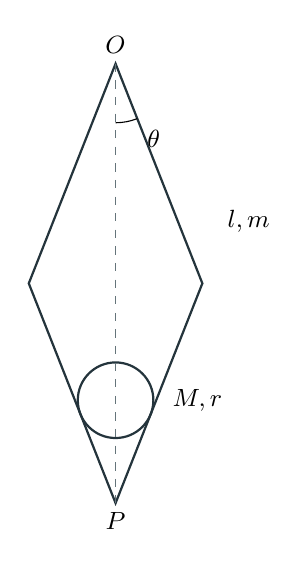
\begin{tikzpicture}
\coordinate(O)at(0,0);\coordinate(P)at(0,-5.580318676994);
\coordinate(U)at(1.102275313068,-2.790159338497);
\coordinate(V)at(-1.102275313068,-2.790159338497);
\coordinate(Cone)at(0,-2.790159338497);\coordinate(Ctwo)at(0,-4.273929989042);
\draw[object](O)--(U)--(P)--(V)--cycle;\draw[object](Ctwo)circle(.48);
\draw[guide](O)--(P);\node[above]at(O){$O$};\node[below]at(P){$P$};
\draw(0,-.75)arc(-90:-68.443095814:.75);\node[right]at(.28,-.95){$\theta$};
\node[right]at(.6,-4.273929989042){$M,r$};\node[right]at(1.3,-2){$l,m$};
\end{tikzpicture}
\figcaption{图5.11\quad 四边均长$l$，圆盘与下方两杆相切，角$\theta$相对竖直方向量起。}\end{minipage}\end{center}

\Needspace{5\baselineskip}\subsection*{解答}

\textbf{用一个角表示两个重心。}以悬点 $O$ 为原点，高度向上为正。由左右对称，四杆的合重心 $C_1$ 在菱形的水平对角线上，距 $O$ 的深度为 $l\cos\theta$；下顶点 $P$ 的深度为 $2l\cos\theta$。
\begin{center}\begin{minipage}{\linewidth}\centering
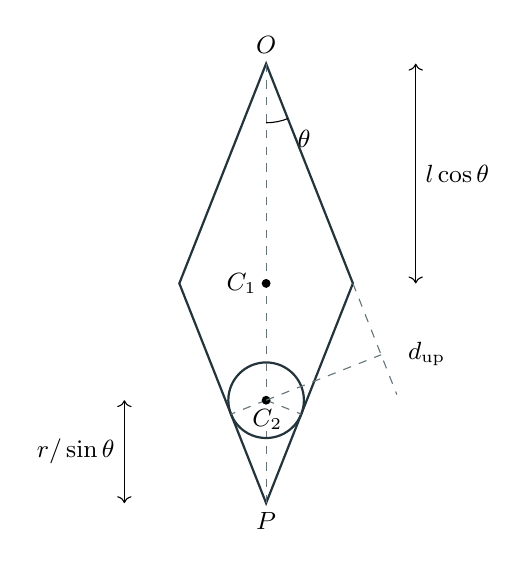
\begin{tikzpicture}
\coordinate(O)at(0,0);\coordinate(P)at(0,-5.580318676994);
\coordinate(U)at(1.102275313068,-2.790159338497);
\coordinate(V)at(-1.102275313068,-2.790159338497);
\coordinate(Cone)at(0,-2.790159338497);\coordinate(Ctwo)at(0,-4.273929989042);
\draw[object](O)--(U)--(P)--(V)--cycle;\draw[object](Ctwo)circle(.48);
\draw[guide](O)--(P);\node[above]at(O){$O$};\node[below]at(P){$P$};
\draw(0,-.75)arc(-90:-68.443095814:.75);\node[right]at(.28,-.95){$\theta$};
\coordinate(K)at(.446425494160,-4.450294039133);
\draw[guide](Ctwo)--(K);\draw[guide](Ctwo)--(-.446425494160,-4.450294039133);
\fill(Cone)circle(1.6pt)node[left]{$C_1$};\fill(Ctwo)circle(1.6pt);
\node[fill=white,inner sep=.7pt]at(.015,-4.52){$C_2$};
\draw[guide](U)--(1.66,-4.201979);
\draw[guide](Ctwo)--(1.460508136,-3.696944281);
\node[anchor=west]at(1.68,-3.69){$d_{\rm up}$};
\draw[<->](1.9,0)--(1.9,-2.790159338497)node[midway,right]{$l\cos\theta$};
\draw[<->](-1.8,-5.580318676994)--(-1.8,-4.273929989042)node[midway,left]{$r/\sin\theta$};
\end{tikzpicture}
\figcaption{解图5.11A\quad 同一数值解的等长菱形与相切圆盘；四杆合重心$C_1$、盘心$C_2$分别标明。}\end{minipage}\end{center}
解图5.11A中，圆盘中心 $C_2$ 在竖直对角线上。它到每根下方木条的垂直距离为 $r$，所以
\[
 PC_2\sin\theta=r,\qquad PC_2=\frac r{\sin\theta}.
\]
两重心的高度为
\[
 y_1=-l\cos\theta,\qquad
 y_2=-2l\cos\theta+\frac r{\sin\theta}.
\]
整体包含四根杆和圆盘；接触力、铰链力为内力，光滑约束允许用重力势能的驻值求平衡。

\textbf{写出势能并求导。}
\begin{align*}
 U&=4mg y_1+Mg y_2\\
  &=-g(4m+2M)l\cos\theta+Mgr\csc\theta,\\
 \frac{\dd U}{\dd\theta}
  &=g(4m+2M)l\sin\theta
    -Mgr\frac{\cos\theta}{\sin^2\theta}.
\end{align*}
故平衡条件为
\[
 (4m+2M)l\sin^3\theta=Mr\cos\theta.\tag{1}
\]
记 $A=(4m+2M)l$、$B=Mr$。$0<\theta<\pi/2$ 时
\[
 \frac1g\frac{\dd^2U}{\dd\theta^2}
 =A\cos\theta+\frac{B}{\sin\theta}
    +\frac{2B\cos^2\theta}{\sin^3\theta}>0.
\]
势能严格凸，驻值是唯一极小，因而在接触模型内稳定。

\textbf{单位换算与数值。}代入国际单位：
\[
 l=0.50\,\mathrm m,\quad m=0.050\,\mathrm{kg},\quad
 r=0.080\,\mathrm m,\quad M=0.200\,\mathrm{kg},
\]
得到 $A=0.300\,\mathrm{kg\,m}$、$B=0.0160\,\mathrm{kg\,m}$。令 $u=\tan\theta>0$，(1)变为
\[
 Au^3=B(1+u^2),\qquad 18.75u^3-u^2-1=0.
\]
可用迭代
\[
 u_{k+1}=u_k-\frac{18.75u_k^3-u_k^2-1}{56.25u_k^2-2u_k}
\]
从 $u_0=0.40$ 出发，迭代值依次为
\[
 u_0=0.400000,\qquad u_1=0.395122,\qquad u_2=0.395058.
\]
第三次迭代已在所列六位小数内不变，于是
\[
 \boxed{\theta\simeq21.557^\circ}.
\]
\begin{center}\begin{minipage}{\linewidth}\centering
\begin{tikzpicture}
\coordinate(P)at(0,0);\coordinate(C)at(0,1.306388687952);
\coordinate(K)at(.446425494160,1.130024637861);
\coordinate(J)at(-.446425494160,1.130024637861);
\draw[object](P)--(1.102275313068,2.790159338497);
\draw[object](P)--(-1.102275313068,2.790159338497);
\draw[object](C)circle(.48);\draw[guide](P)--(C)--(K);\draw[guide](C)--(J);
\draw[force](K)--(-.819204883,1.630024637861)node[left]{$N$};
\draw[force](J)--(.819204883,1.630024637861)node[right]{$N$};
\draw[force](C)--(0,.306388687952)node[below right]{$Mg$};
\fill(K)circle(1.7pt)node[right]{$K$};\fill(C)circle(1.4pt);
\draw[guide](C)--(0,1.9);\node[above]at(0,1.9){$C_2$};
\node[below]at(P){$P$};\node[below]at(.22,1.2){$r$};
\node[align=left,anchor=west]at(1.5,.65){$PK=r\cot\theta<l$\\接触点位于杆内};
\end{tikzpicture}
\figcaption{解图5.11B\quad 两条法向力作用线均通过盘心，竖直分量合成盘重；半径$C_2K$与木条垂直。}
\end{minipage}\end{center}
\textbf{圆盘切点与木条的间隙。}解图5.11B的切点 $K$ 到下顶点的距离为 $PK=r\cot\theta$，代入得约 $0.2025\,\mathrm m<l$，切点在杆内。

解图5.11A中，圆盘与上方木条留有间隙时，盘心到上方木条所在直线的距离 $d_{\rm up}=2l\sin\theta\cos\theta-r$ 大于半径 $r$，等于 $r$ 时恰好相切。两种情形合写为
\[
 r\le l\sin\theta\cos\theta.
\]
计算右端约为 $0.1709\,\mathrm m>0.080\,\mathrm m$，满足要求。两侧法向力的竖直分量平衡圆盘重力：
\[
 2N\sin\theta=Mg,\qquad N=\frac{Mg}{2\sin\theta}>0.
\]
因此圆盘由两根下杆支承，两切点均在杆内，圆盘与上杆之间有间隙。
\subsubsection*{系统质心、平衡角和接触力}
把四杆合重心与盘心合并，系统质心高度明确写为
\[
y_C=\frac{4my_1+My_2}{4m+M}
=-\frac{(4m+2M)l\cos\theta-Mr\csc\theta}{4m+M}.
\]
乘以总质量和 $g$ 得到前面的势能。菱形张开时，圆盘的高度同时随下顶点的位置和盘心到下顶点的相切距离变化，两项都进入势能。

将质量和长度换成统一单位后，数值方程的系数为
\[
\frac{(4m+2M)l}{Mr}=\frac{0.300}{0.0160}=18.75,
\]
\[
u_*=0.395058195372\ldots,\qquad
\theta=21.55690419^\circ.
\]
因此$PK=r/u_*=0.20250181\,\mathrm m$，
盘心到上杆直线的距离为
$2l\sin\theta\cos\theta-r=0.26172486\,\mathrm m>r$。
以上两段距离都用平衡角 $\theta$ 求得。解图5.11A、B 取相同的 $l:r$ 和同一个平衡角。
每一接触法向力的大小为$N=1.36082155\,Mg$，为正，
其两竖直分量之和恰为$Mg$，水平分量相消。

平衡方程也可写为
\[
\frac{\sin^3\theta}{\cos\theta}
=\frac{Mr}{(4m+2M)l}.
\]
左侧在$0<\theta<\pi/2$中导数为
$3\sin^2\theta+\sin^4\theta/\cos^2\theta>0$，
从零增加到无穷，因此只有一个数学驻值。
驻值是否对应两根下杆支承圆盘，由切点是否落在杆上以及圆盘与上杆的间隙确定。

\subsubsection*{整体摆动自由度的判稳}
前面得到的正曲率对应机构张角$\theta$的变化。
若还允许整个菱形在平面内偏离竖直角$\psi$，
组合重心仍在其对称轴上，故重力势能为
\[
U(\theta,\psi)=U_0(\theta)\cos\psi,
\qquad
U_0(\theta)=-g[(4m+2M)l\cos\theta-Mr\csc\theta].
\]
在求得的构型中$U_0<0$，即组合重心位于悬点下方。
在$\psi=0,U_0'(\theta_*)=0$处，
\[
U_{\theta\theta}=U_0''(\theta_*)>0,\qquad
U_{\psi\psi}=-U_0(\theta_*)>0,\qquad
U_{\theta\psi}=0.
\]
所以机构张合与整体摆动两种小偏离均有恢复趋势，
张角与整体转角这两个平面自由度的势能曲率均为正。
这个判断仍建立在圆盘继续由下方两杆光滑接触的构型内。


\Needspace{18\baselineskip}

\pdfbookmark[2]{第 12 题 细绳张力与悬链线}{q12}

\section*{第 12 题\quad 细绳张力与悬链线}

\tagline{M-05-12}

质量分布均匀的柔软细绳长 $L$，线密度为 $\lambda$，静止悬于两个竖直支杆。两端向上的切线与竖直方向的夹角分别为 $\theta_1,\theta_2$，$0<\theta_1,\theta_2<\pi/2$。取左支杆为 $y$ 轴，水平向右为 $x$ 轴，左悬点为 $(0,H)$。
\begin{enumerate}\item 求两端张力。\item 推导悬链线方程，确定全部积分常量，并由所得方程求两端斜率和整段弧长。\end{enumerate}

\begin{center}\begin{minipage}{\linewidth}\centering
\begin{tikzpicture}
\draw[axis](0,-.2)--(0,3.9)node[above]{$y$};
\draw[axis](-.2,0)--(5.65,0)node[right]{$x$};\draw[object](5,0)--(5,3.3);
\draw[traj,domain=0:5,samples=110]plot(\x,{.5+2.2*(cosh((\x-2.2)/2.2)-1)});
\coordinate(A)at(0,1.694777396594);\coordinate(B)at(5,2.535708393558);
\fill(A)circle(1.7pt);\fill(B)circle(1.7pt);\node[left]at(A){$(0,H)$};
\draw[guide](A)--(-.65,2.458658172462);
\draw[guide](B)--(5.6,3.522861535308);
\draw(0,2.201777396594)arc(90:130.395062579:.507);
\node at(-.43,2.47){$\theta_1$};
\draw(5,3.042708393558)arc(90:58.708413156:.507);
\node at(5.27,3.3){$\theta_2$};
\node at(2.5,.15){全长$L$，线密度$\lambda$};
\end{tikzpicture}
\figcaption{图5.12\quad 两端均向上悬挂，$\theta_1,\theta_2$分别在端点切线与竖直线之间量取。}\end{minipage}\end{center}

\Needspace{5\baselineskip}\subsection*{解答}

\textbf{整绳平衡确定端点张力。}解图5.12A的 $\theta_1,\theta_2$ 都相对竖直量起。两端水平分量相等，竖直分量共同承受绳重：
\[
 T_1\sin\theta_1=T_2\sin\theta_2=:K,\qquad
 T_1\cos\theta_1+T_2\cos\theta_2=\lambda gL.
\]
所以 $K(\cot\theta_1+\cot\theta_2)=\lambda gL$。化简得
\[
 \boxed{T_1=\frac{\lambda gL\sin\theta_2}{\sin(\theta_1+\theta_2)}},
 \qquad
 \boxed{T_2=\frac{\lambda gL\sin\theta_1}{\sin(\theta_1+\theta_2)}}.
\]
\begin{center}\begin{minipage}{\linewidth}\centering
\begin{tikzpicture}
\draw[axis](0,-.2)--(0,3.9)node[above]{$y$};
\draw[axis](-.2,0)--(5.65,0)node[right]{$x$};\draw[object](5,0)--(5,3.3);
\draw[traj,domain=0:5,samples=110]plot(\x,{.5+2.2*(cosh((\x-2.2)/2.2)-1)});
\coordinate(A)at(0,1.694777396594);\coordinate(B)at(5,2.535708393558);
\fill(A)circle(1.7pt);\fill(B)circle(1.7pt);\node[left]at(A){$(0,H)$};
\draw[guide](A)--(-.65,2.458658172462);
\draw[guide](B)--(5.6,3.522861535308);
\draw(0,2.201777396594)arc(90:130.395062579:.507);
\node at(-.43,2.47){$\theta_1$};
\draw(5,3.042708393558)arc(90:58.708413156:.507);
\node at(5.27,3.3){$\theta_2$};
\draw[force](A)--(-.7,2.517418232144)node[left]{$T_1$};
\draw[force](B)--(5.7,3.687387058933)node[right]{$T_2$};
\fill(2.618492916965,1.129039954884)circle(1.6pt)node[above left]{$C_G$};
\draw[force](2.618492916965,1.129039954884)--(2.618492916965,-.845279546042)node[right]{$\lambda gL$};
\node at(2.5,-1.5){全长$L$，线密度$\lambda$};
\end{tikzpicture}
\figcaption{解图5.12A\quad 端张力沿实际切线，两个水平分量同为$K$；绳重铅垂线通过同一曲线的重心。}\end{minipage}\end{center}
\textbf{定义局部角并建立微元方程。}沿绳从左向右取弧长 $s$，将横坐标 $x$ 处切线与 $x$ 轴正向的夹角记为 $\varphi(x)$，$-\pi/2<\varphi<\pi/2$。左端切线向右下方，因此
\[
 \varphi(0)=\theta_1-\frac\pi2;
\]
右端切线向右上方，因此 $\varphi(b)=\pi/2-\theta_2$。局部$\varphi$从水平量且保留正负，两端$\theta_i$从向上竖直方向量，按上述互余关系换算。
\begin{center}\begin{minipage}{\linewidth}\centering
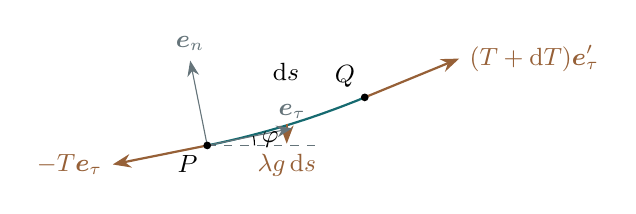
\begin{tikzpicture}
\coordinate(P)at(0,0);\coordinate(Q)at(2,.610056162194);
\draw[traj,domain=0:2,samples=80]plot(\x,{10*(cosh((\x+2)/10)-cosh(.2))});
\draw[force](P)--(-1.2,-.241603203049)node[left]{$-T\vect e_\tau$};
\draw[force](Q)--(3.2,1.102958953157)node[right]{$(T+\dd T)\vect e_\tau'$};
\draw[force](1.009703952961,.273129838393)--(1.009703952961,.021830250479)node[below]{$\lambda g\dd s$};
\draw[axis](P)--(1.078361262411,.217112852248)node[above]{$\vect e_\tau$};
\draw[axis](P)--(-.217112852248,1.078361262411)node[above]{$\vect e_n$};
\draw[guide](P)--(1.4,0);\draw(.6,0)arc(0:11.383516663:.6);
\node at(.8,.075){$\varphi$};\node[above]at(1,.7){$\dd s$};
\fill(P)circle(1.4pt)node[below left]{$P$};\fill(Q)circle(1.4pt)node[above left]{$Q$};
\end{tikzpicture}
\figcaption{解图5.12B\quad 右支绳元从$P$到$Q$，局部角从水平量起；两端张力分别沿各自切线。}
\end{minipage}\end{center}
按解图5.12B中有符号的切线角，对长度 $\dd s$ 的绳元取切向、法向平衡。切向单位矢量为 $(\cos\varphi,\sin\varphi)$，法向为 $(-\sin\varphi,\cos\varphi)$，重力为 $(0,-\lambda g\dd s)$，故
\[
 \frac{\dd T}{\dd s}=\lambda g\sin\varphi,\qquad
 T\frac{\dd\varphi}{\dd s}=\lambda g\cos\varphi.\tag{1}
\]
将两式相除：$\dd T/T=\tan\varphi\dd\varphi$，积分得
\[
 T\cos\varphi=K.\tag{2}
\]
$K$ 正是整绳平衡中的恒定水平张力，由各端张力的水平分量共同确定。设
\[
 a=\frac K{\lambda g}
 =\frac{L}{\cot\theta_1+\cot\theta_2}>0.\tag{3}
\]
\textbf{先积分高度关系。}因 $\dd y/\dd s=\sin\varphi$，(1)第一式给出
\[
 \dd T=\lambda g\dd y,\qquad T=\lambda gy+C_2.
\]
用左端 $y=H,T=T_1$ 确定 $C_2=T_1-\lambda gH$，因此
\[
 y=H+\frac{T-T_1}{\lambda g}.\tag{4}
\]
\textbf{再积分水平位置。}由 $\dd x/\dd s=\cos\varphi$，(1)第二式成为 $T\dd\varphi=\lambda g\dd x$。代入(2)：
\[
 \dd x=a\sec\varphi\dd\varphi,
 \quad x=a\ln(\sec\varphi+\tan\varphi)+x_0
 =a\operatorname{arsinh}(\tan\varphi)+x_0.
\]
反双曲正弦是奇函数。左支的 $\tan\varphi<0$ 给 $x<x_0$，右支的 $\tan\varphi>0$ 给 $x>x_0$。

左端 $x=0$、$\tan\varphi=-\cot\theta_1$，故
\[
 x_0=a\operatorname{arsinh}(\cot\theta_1)>0.
\]
反解得 $\tan\varphi=\sinh((x-x_0)/a)$，于是
\[
 T=K\sec\varphi=K\cosh\frac{x-x_0}{a}.
\]
又 $T_1=K\csc\theta_1$，代入(4)得到完整方程
\[
 \boxed{y(x)=H+a\left[\cosh\frac{x-x_0}{a}-\csc\theta_1\right]},
 \qquad \boxed{x_0=a\operatorname{arsinh}(\cot\theta_1)}.
\]
\begin{center}\begin{minipage}{\linewidth}\centering
\begin{tikzpicture}
\draw[axis](-.4,0)--(5.9,0)node[right]{$x$};
\draw[axis](0,-.2)--(0,3.5)node[above]{$y$};
\draw[traj,domain=0:5,samples=110]plot(\x,{.5+2.2*(cosh((\x-2.2)/2.2)-1)});
\draw[guide](2.2,0)--(2.2,3);\fill(2.2,.5)circle(1.7pt);
\node[below]at(2.2,0){$x_0$};\node[above]at(2.2,.5){最低点};
\node[left]at(0,1.694777396594){$H$};
\draw[guide](0,.5)--(2.2,.5);\node[left]at(0,.5){$y_0$};
\fill(5,2.535708393558)circle(1.7pt)node[right]{$x=b$};
\draw[<->](0,-.65)--(2.2,-.65)node[midway,below]{$a\operatorname{arsinh}(\cot\theta_1)$};
\end{tikzpicture}
\figcaption{解图5.12C\quad 与解图5.12A同一组曲线参数；最低点、端点、跨度及高度统一标注。}
\end{minipage}\end{center}
\textbf{最低点、端点斜率与弧长。}解图5.12C中，最低点在 $x=x_0$，高度为 $y_0=H-a(\csc\theta_1-1)$。求导：
\[
 y'=\sinh\frac{x-x_0}{a}.
\]
左端 $y'(0)=-\cot\theta_1$，方向为向右下方；右端 $y'(b)=\cot\theta_2$，因此跨度和右端高度为
\[
 b=a\bigl[\operatorname{arsinh}(\cot\theta_1)
          +\operatorname{arsinh}(\cot\theta_2)\bigr],
\]
\[
 y(b)=H+a(\csc\theta_2-\csc\theta_1).
\]
从左端到右端沿曲线积分，得到整根绳的弧长，
\begin{align*}
 \int_0^b\sqrt{1+y'^2}\dd x
 &=\int_0^b\cosh\frac{x-x_0}{a}\dd x\\
 &=a\left[\sinh\frac{b-x_0}{a}-\sinh\frac{-x_0}{a}\right]\\
 &=a(\cot\theta_2+\cot\theta_1)=L.
\end{align*}
代回张力 $T=K\sqrt{1+y'^2}$，两端也恢复 $T_1,T_2$。

\textbf{另解：直角坐标微元。}绳的张力向量可写为 $(K,Ky')$，长度微元 $\dd s=\sqrt{1+y'^2}\dd x$。竖直平衡给出
\[
 K y''\dd x=\lambda g\sqrt{1+y'^2}\dd x,
 \quad \frac{y''}{\sqrt{1+y'^2}}=\frac1a.
\]
第一次积分：$\operatorname{arsinh}y'=(x-x_0)/a$；第二次积分：$y=y_0+a[\cosh((x-x_0)/a)-1]$。由左端高度和斜率确定同样的 $x_0,y_0$。
\subsubsection*{自然坐标微元式中的一阶项}
解图5.12B取右支局部放大图，$\varphi>0$；沿$P$到$Q$张力增加。
在左支同一有符号方程仍成立，只是$\varphi<0$时$\dd T<0$。
投影中的$\varphi$取微元中点；在微元极限下，它与图示$P$处切线角的差只影响已舍去的高阶项。
为看清张力方向改变的贡献，可先把两端张力投到弧元中点的切、法线：
\[
\dd T\cos\frac{\dd\varphi}{2}
=\lambda g\dd s\sin\varphi,
\]
\[
(2T+\dd T)\sin\frac{\dd\varphi}{2}
=\lambda g\dd s\cos\varphi.
\]
利用$\cos(\dd\varphi/2)=1+O(\dd\varphi^2)$、
$\sin(\dd\varphi/2)=\dd\varphi/2+O(\dd\varphi^3)$，
并舍去$\dd T\,\dd\varphi$这类二阶微量，
恰恢复式(1)的两条微分方程。
法向式中的张力合力来自切线方向改变；两端大小接近时，法向分量仍以$T\dd\varphi$的一阶量相加。

相除后积分的中间计算为
\[
\int\frac{\dd T}{T}
=\int\tan\varphi\,\dd\varphi
=-\ln(\cos\varphi)+\ln K.
\]
因局部切线始终朝右，$\cos\varphi>0$，故$T\cos\varphi=K>0$。
左端切线角 $\varphi_A$ 为负，右端 $\varphi_B$ 为正。各端水平倾角的绝对值与相应竖直夹角互余，所以 $\cos\varphi_A=\sin\theta_1$、$\cos\varphi_B=\sin\theta_2$。
反双曲正弦为奇函数，左支给负值、右支给正值，
因此两个有符号分支在最低点平滑接合，积分常量的平移方向由左端条件确定。

\subsubsection*{从最低点弧长重建张力与端点}
令$\sigma$为从最低点起算、向右为正的有符号弧长。
积分$\dd\sigma=\cosh[(x-x_0)/a]\dd x$得
\[
\sigma=a\sinh\frac{x-x_0}{a},\qquad
T_y=Ky'=\lambda g\sigma,
\]
\[
T=\sqrt{K^2+(\lambda g\sigma)^2}.
\]
这表示局部张力的竖直分量等于最低点至该位置一段绳的有符号重量，
左侧负、右侧正。两端到最低点的弧长大小分别为
\[
L_1=a\cot\theta_1,\qquad L_2=a\cot\theta_2,\qquad
L_1+L_2=L.
\]
式(3)于是也可从弧长分配直接恢复。
最低点 $\sigma=0$ 给 $T_{\min}=K$。从最低点向任一端走，$|\sigma|$ 和张力都增大，
并且$T-T_{\min}=\lambda g(y-y_0)$与高度积分式一致。

曲率可用悬链线的两个导数表示，
\[
\kappa=\frac{y''}{(1+y'^2)^{3/2}}
=\frac1{a\cosh^2[(x-x_0)/a]}.
\]
最低点的曲率半径为$a$，两侧曲率减小。
二阶导数$y''=\cosh[(x-x_0)/a]/a$却向两侧增加，
曲率还含斜率因子$(1+y^{\prime2})^{-3/2}$，两种量因而有不同的变化趋势。

题中$L,\theta_1,\theta_2,H$已确定$a,x_0,y_0$，
也就确定了跨度$b$与右端高度。
额外给出的跨度或右端高度，取值应满足由这四个已知量推得的关系。
解图5.12A、C统一用同一组$a=2.2,x_0=2.2,b=5,y_0=0.5$的示例，
相应$L=6.20500415$，两个竖直端角约为$40.3951^\circ$和$31.2916^\circ$；
曲线端点、切线方向和整绳重心$C_G$的铅垂线都依同一参数计算。


\end{document}
